\documentclass[11pt]{beamer}

\usepackage[utf8]{inputenc}
\usepackage{xcolor}
\usepackage{caption}
\usepackage[natbibapa]{apacite}
\usepackage{bbm}
\bibliographystyle{apacite}
\renewcommand{\bibsection}{\subsubsection*{\bibname}}
\renewcommand*{\bibfont}{\scriptsize}

\usepackage{pgfplots}
\usepackage{tikz}
\usepackage{subcaption}

\pgfplotsset{compat=1.16}


\usetheme{Ilmenau}
\usecolortheme{lily}
\newcommand{\light}[2][35]{\color{fg!#1}#2}

\DeclareMathOperator*{\argmin}{arg\,min}

% Nicer looking Itemize and enumerate environments
\newenvironment{wideitemize}{\itemize\addtolength{\itemsep}{14pt}}{\enditemize}
\newenvironment{widenumerate}{\enumerate\addtolength{\itemsep}{14pt}}{\endenumerate}


\defbeamertemplate*{footline}{myminiframes theme}
  {%
    \begin{beamercolorbox}[colsep=1.5pt]{upper separation line foot}
    \end{beamercolorbox}
    \begin{beamercolorbox}[ht=2.5ex,dp=1.125ex,%
      leftskip=.3cm,rightskip=.3cm plus1fil]{author in head/foot}%
      \leavevmode{\usebeamerfont{author in head/foot}\insertshortauthor}%
      \hfill%
      {\usebeamerfont{institute in head/foot}\usebeamercolor[fg]{institute in head/foot}\insertshortinstitute}%
    \end{beamercolorbox}%
    \begin{beamercolorbox}[ht=2.5ex,dp=1.125ex,%
      leftskip=.3cm,rightskip=.3cm plus1fil]{title in head/foot}%
      {\usebeamerfont{title in head/foot}\insertshorttitle\hfill \insertframenumber/\inserttotalframenumber}%<-here
    \end{beamercolorbox}%
    \begin{beamercolorbox}[colsep=1.5pt]{lower separation line foot}
    \end{beamercolorbox}
}





\title{From Value Added to Welfare Added}
\author{
Tanner S Eastmond\inst{1} \and Nathan Mather\inst{2} \and Michael Ricks\inst{3}} 
\date{\vspace{-8ex}}
\institute[]{\inst{1}Department of Economics, University of California San Diego, \and \inst{2}Department of Economics, University of Michigan}
\date{}

\begin{document}




%%%%%%%%%%%%%%%%%%%%%%%%%%%%%%%%%%%%%%%%%%%%%%%%%%%%%%%%
%%%%%%%%%%%%%%%%%%%%%% Tile Page. %%%%%%%%%%%%%%%%%%%%%%
%%%%%%%%%%%%%%%%%%%%%%%%%%%%%%%%%%%%%%%%%%%%%%%%%%%%%%%%

\begin{frame}
    \maketitle
\end{frame}




%%%%%%%%%%%%%%%%%%%%%%%%%%%%%%%%%%%%%%%%%%%%%%%%%%%%%%%%
%%%%%%%%%%%%%%%%%%%%% Introduction %%%%%%%%%%%%%%%%%%%%%
%%%%%%%%%%%%%%%%%%%%%%%%%%%%%%%%%%%%%%%%%%%%%%%%%%%%%%%%

\section{Introduction}

%%%%%%%%%%%%%%%%%%%%%%%%%%%%%%%%%%%%%%%%%%%%%%%%%%%%%%%%
%%%%%%%%%%%%%%%%%%%%%%%%%%%%%%%%%%%%%%%%%%%%%%%%%%%%%%%%

\begin{frame}{Value Added Measures: The Goal}

\begin{itemize}
    \item Goal of Value added measures (VAM) are to rank teachers' ``effectiveness''
        \begin{itemize}
            \item Measure post test achievement controlling for a pretest score
        \end{itemize}
    \item VAM do capture something real
    \begin{itemize}
        \item {\color{gray}{\citep{chetty2014measuring2, pope2017multidimensional}}}
    \end{itemize}
    \item There is heterogeneity in test score effects VAM do not catch
    \begin{itemize}
        \item {\color{gray}{\citep{ehrenberg1995teachers, dee2005teacher, lockwood2009}}}
    \end{itemize}
\end{itemize}

\end{frame}


%%%%%%%%%%%%%%%%%%%%%%%%%%%%%%%%%%%%%%%%%%%%%%%%%%%%%%%%
%%%%%%%%%%%%%%%%%%%%%%%%%%%%%%%%%%%%%%%%%%%%%%%%%%%%%%%%

\begin{frame}{Value Added Measures: A Policy Disconnect}

\begin{itemize}
    \item Theoretical disconnect between education policy goals and use of VAM 
    \begin{itemize}
        \item Policies explicitly target gains in some subpopulations
        \item VAM are mean-oriented statistics: a teacher's average impact on students' scores
        \item Resulting VAM rankings may carry different \textbf{implicit normative} ``welfare weights''
    \end{itemize}
    
    \item  We propose a set of more flexible heterogeneous VAM 
    \begin{itemize}
        \item Assess teachers' heterogeneous impacts along the achievement distribution
        \item  Weight effects according to an \textbf{explicit normative} policy goal or welfare criterion
    \end{itemize}
\end{itemize}

\end{frame}


%%%%%%%%%%%%%%%%%%%%%%%%%%%%%%%%%%%%%%%%%%%%%%%%%%%%%%%%
%%%%%%%%%%%%%%%%%%%%%%%%%%%%%%%%%%%%%%%%%%%%%%%%%%%%%%%%

\begin{frame}{Research Goals}

\begin{enumerate}
    \item Build a welfare-relevant framework for VAM (and other educational statistics) 
    \item Propose methods to estimate value added over the achievement distribution
    \item Explore feasibility and accuracy of methods in simulations
    \item Estimate VA heterogeneity and welfare implications in real student-teacher data
\end{enumerate}
\end{frame}




%%%%%%%%%%%%%%%%%%%%%%%%%%%%%%%%%%%%%%%%%%%%%%%%%%%%%%%%
%%%%%%%%%%%%%%%%%%%%%%%% Methods %%%%%%%%%%%%%%%%%%%%%%%
%%%%%%%%%%%%%%%%%%%%%%%%%%%%%%%%%%%%%%%%%%%%%%%%%%%%%%%%

\section{Methods}

%%%%%%%%%%%%%%%%%%%%%%%%%%%%%%%%%%%%%%%%%%%%%%%%%%%%%%%%
%%%%%%%%%%%%%%%%%%%%%%%%%%%%%%%%%%%%%%%%%%%%%%%%%%%%%%%%

\begin{frame}{Estimating Standard  Value Added}

\begin{itemize}
    \item In theory test scores are a function of testing ability, value added, and noise
    \begin{align*}
    y_{ijt}  &= a_{it} + \epsilon_{ijt} \\
    y_{ijt}  &= a_{it-1} + VA_j(a_{it-1}) + \epsilon_{ijt}
    \end{align*}
 
    \item We don't observe testing ability. Traditional VAM assumptions:
    \begin{itemize}
        \item Predict testing ability with characteristics (including lagged scores): $X_{it}$
        \item Assume homogeneity within and across teachers $VA_j(\cdot)=\gamma_j$ with no $ij$ error
    \end{itemize}
    \begin{align*}
    y_{ijt}  &= \beta X_{it} +\Gamma D_{it} +\mu_{jt} + \eta_{it}
    \end{align*}
    
    \item Note the $\mu_{jt}$ variation could pick up $ij$ variation.
       
    
\end{itemize}
\end{frame}


%%%%%%%%%%%%%%%%%%%%%%%%%%%%%%%%%%%%%%%%%%%%%%%%%%%%%%%%
%%%%%%%%%%%%%%%%%%%%%%%%%%%%%%%%%%%%%%%%%%%%%%%%%%%%%%%%

\begin{frame}{Modeling Value Added As Social Welfare}

\begin{itemize}
    \item We can think of the following social welfare function
    \begin{itemize}
        \item $\omega(x_i,y_i)$ weights: likely based on \textit{ex ante} expected performance
        % Talk about the concavity here?
        \item $v(x_i,y_i)$ value: think achievement, gains, etc.
    \end{itemize}
    \[
    W  = \sum_i \omega(x_i,y_i) v(x_i,y_i) 
    \] 
    
    \item Traditional VAM take the average gains for students among each teacher
    \begin{itemize}
        \item Let $x_i$ be \textit{ex ante} expected performance, estimated as $\hat{y}_i$, then $\tilde{v}(\cdot) = y_i - \hat{y}_i$
    \end{itemize}
    \[
    \hat{W}_{VA}  = \sum_i \frac{(y_i-\hat{y}_i)}{N_{j(i)}} \hspace{3em}
    \]
    
    \item This implies $\omega(x_i,y_i)=\frac{1}{N_j}$, which is (almost) utilitarian

\end{itemize}


\end{frame}


%%%%%%%%%%%%%%%%%%%%%%%%%%%%%%%%%%%%%%%%%%%%%%%%%%%%%%%%
%%%%%%%%%%%%%%%%%%%%%%%%%%%%%%%%%%%%%%%%%%%%%%%%%%%%%%%%

\begin{frame}{``Welfare Added''}

\begin{itemize}
    \item Let $\hat{v}_j(x_i,y_i)$ estimate a teacher's heterogeneous value added, $\mathbb{E}[v(\cdot)|x_i,j]$
    
    \item Then the estimated ``Welfare Added'' by this teacher is  
    \[
    \hat{W}_j  = \sum_{i\in j} \omega(x_i,y_i) \hat{v}_j(x_i,y_i) 
    \] 
    
    \item Consider the following examples:
    \begin{itemize}
        \item Utilitarian: All students are weighted equally $\omega(x_i,y_i) = 1$
        \item Rawlsian: We care only about students below some cutoff, $c$, $\omega(x_i,y_i) = \mathds{1}(x_i\leq c)$
        \item Pareto: We care about the lower achieving students more $ \omega(x_i,y_i)=  \frac{\alpha x_\mathrm{m}^\alpha}{x_i^{\alpha+1}}$ 
    \end{itemize}
    
    %\item But estimating Welfare Added requires an estimate of $\mathbb{E}[v(\cdot)|x_i,j]$
\end{itemize}


\end{frame}


%%%%%%%%%%%%%%%%%%%%%%%%%%%%%%%%%%%%%%%%%%%%%%%%%%%%%%%%
%%%%%%%%%%%%%%%%%%%%%%%%%%%%%%%%%%%%%%%%%%%%%%%%%%%%%%%%

\begin{frame}{Estimating Effect Heterogeneity}

\begin{itemize}
    \item Intuitively, imagine a pointwise approach for estimating $\hat{v}_j(x_i,y_i)$
    
    \item Binning students by \textit{ex ante} expected score and estimating VA has two problems
    \begin{enumerate}
        \item We don't have infinite data, so bins would be too small
        \item We don't actually know the \textit{ex ante} expected score
    \end{enumerate}

    \item $\hat{y}_{it} = \hat{\beta} X_{it}$ consistently predicts expected score, but with error

\end{itemize}

\end{frame}


%%%%%%%%%%%%%%%%%%%%%%%%%%%%%%%%%%%%%%%%%%%%%%%%%%%%%%%%
%%%%%%%%%%%%%%%%%%%%%%%%%%%%%%%%%%%%%%%%%%%%%%%%%%%%%%%%

\begin{frame}{Estimating Effect Heterogeneity}

    We propose two methods to estimate heterogeneity in VAM across the achievement distribution:
    
    \begin{enumerate}
        \item Standard VA including interacted dummies for prior `ability'
        \item Kernel Regression
    \end{enumerate}
    
\end{frame}




%%%%%%%%%%%%%%%%%%%%%%%%%%%%%%%%%%%%%%%%%%%%%%%%%%%%%%%%
%%%%%%%%%%%%%%%%%%%%%% Simulations %%%%%%%%%%%%%%%%%%%%%
%%%%%%%%%%%%%%%%%%%%%%%%%%%%%%%%%%%%%%%%%%%%%%%%%%%%%%%%

\section{Simulations}

%%%%%%%%%%%%%%%%%%%%%%%%%%%%%%%%%%%%%%%%%%%%%%%%%%%%%%%%
%%%%%%%%%%%%%%%%%%%%%%%%%%%%%%%%%%%%%%%%%%%%%%%%%%%%%%%%

\begin{frame}{Definitions}

    \begin{itemize}
        \item<1-> \textbf{Standard VA} - A teacher's true impact on a typical class of students
        \item<1-> \textbf{Welfare-Weighted VA} - A teacher's true impact on a typical class of students, weighted by the explicit policy goal
        \item<3> \textbf{Standard VA Estimate} - A teacher's estimated mean impact on a typical class of students
        \item<3> \textbf{Alternative VA Estimate} - A teacher's estimated impact on a typical class of students allowing for heterogeneity across the achievement distribution and explicitly applying the welfare weights
    \end{itemize}
    
    \only<2>{These are theoretical benchmarks}

\end{frame}


%%%%%%%%%%%%%%%%%%%%%%%%%%%%%%%%%%%%%%%%%%%%%%%%%%%%%%%%
%%%%%%%%%%%%%%%%%%%%%%%%%%%%%%%%%%%%%%%%%%%%%%%%%%%%%%%%

\begin{frame}{Simulation Setup}

    \only<1>{
        \begin{itemize}
            \item Students have Normally distributed testing ability
            \item Students are randomly assigned to teachers
            \item Our welfare weight in these simulations put 4 times more weight on students below the 40th percentile of prior achievement.
        \end{itemize}
    }

    \includegraphics<2>[width=\textwidth]{slides/Figures/teacher_example_just_truth_1.png}
    
    \includegraphics<3>[width=\textwidth]{slides/Figures/standard_cent_run_just_stand_3.png}
    
    \includegraphics<4>[width=\textwidth]{slides/Figures/standard_cent_run_3.png}

\end{frame}


%%%%%%%%%%%%%%%%%%%%%%%%%%%%%%%%%%%%%%%%%%%%%%%%%%%%%%%%
%%%%%%%%%%%%%%%%%%%%%%%%%%%%%%%%%%%%%%%%%%%%%%%%%%%%%%%%

\begin{frame}{How much does heterogeneity in match quality matter?}

    \only<1>{
        We can imagine a situation where teachers do impact students like the example given above, but that difference in overall teacher ability swamp match quality.
    }
    
    \only<2>{
    Consider two `dimensions' where teachers may differ in their Welfare-Weighted VA:
    \begin{enumerate}
        \item Overall teacher ability
        \item Match quality with students at other points in the achievement distribution
    \end{enumerate}
    }

\end{frame}


%%%%%%%%%%%%%%%%%%%%%%%%%%%%%%%%%%%%%%%%%%%%%%%%%%%%%%%%
%%%%%%%%%%%%%%%%%%%%%%%%%%%%%%%%%%%%%%%%%%%%%%%%%%%%%%%%

\begin{frame}{Only Variation in Teacher Ability}

    \hypertarget<1>{teacher_ability1}{}
    \hypertarget<2>{teacher_ability2}{}
    
    \includegraphics<1>[width=\textwidth]{slides/Figures/standard_cat_run_1.png}
    \includegraphics<2>[width=\textwidth]{slides/Figures/np_ww_cat_run_1.png}
    \includegraphics<3>[width=\textwidth]{slides/Figures/np_hist_run_1.png}
    
    \hyperlink<1>{st_cent1}{\beamerbutton{Standard Match Quality}}
    \hyperlink<2->{np_cent1}{\beamerbutton{NP Match Quality}}
    \hyperlink<3>{st_cent1}{\beamerbutton{Standard Match Quality}}

\end{frame}


%%%%%%%%%%%%%%%%%%%%%%%%%%%%%%%%%%%%%%%%%%%%%%%%%%%%%%%%
%%%%%%%%%%%%%%%%%%%%%%%%%%%%%%%%%%%%%%%%%%%%%%%%%%%%%%%%

%\begin{frame}{Only Variation in Match Quality with Average Students}

%    \hypertarget<1>{match_average1}{}
%    \hypertarget<2>{match_average2}{}
    
%    \includegraphics<1>[width=\textwidth]{slides/Figures/standard_cat_run_2.png}
%    \includegraphics<2>[width=\textwidth]{slides/Figures/np_ww_cat_run_2.png}
%    \includegraphics<3>[width=\textwidth]{slides/Figures/np_hist_run_2.png}
    
%    \hyperlink<1>{st_cent2}{\beamerbutton{Standard Match Quality}}
%    \hyperlink<2->{np_cent2}{\beamerbutton{NP Match Quality}}
%    \hyperlink<3>{st_cent2}{\beamerbutton{Standard Match Quality}}

%\end{frame}


%%%%%%%%%%%%%%%%%%%%%%%%%%%%%%%%%%%%%%%%%%%%%%%%%%%%%%%%
%%%%%%%%%%%%%%%%%%%%%%%%%%%%%%%%%%%%%%%%%%%%%%%%%%%%%%%%

\begin{frame}{Only Variation in Match Quality}

    \hypertarget<1>{match_quality1}{}
    \hypertarget<2>{match_quality2}{}
    
    \includegraphics<1>[width=\textwidth]{slides/Figures/standard_cat_run_3.png}
    \includegraphics<2>[width=\textwidth]{slides/Figures/np_ww_cat_run_3.png}
    \includegraphics<3>[width=\textwidth]{slides/Figures/np_hist_run_3.png}
    
    \hyperlink<1>{st_cent3}{\beamerbutton{Standard Match Quality}}
    \hyperlink<2->{np_cent3}{\beamerbutton{NP Match Quality}}
    \hyperlink<3>{st_cent3}{\beamerbutton{Standard Match Quality}}

\end{frame}


%%%%%%%%%%%%%%%%%%%%%%%%%%%%%%%%%%%%%%%%%%%%%%%%%%%%%%%%
%%%%%%%%%%%%%%%%%%%%%%%%%%%%%%%%%%%%%%%%%%%%%%%%%%%%%%%%

\begin{frame}{Variation in All}

    \hypertarget<1>{all1}{}
    \hypertarget<2>{all2}{}
    
    \includegraphics<1>[width=\textwidth]{slides/Figures/standard_cat_run_4.png}
    \includegraphics<2>[width=\textwidth]{slides/Figures/np_ww_cat_run_4.png}
    \includegraphics<3>[width=\textwidth]{slides/Figures/np_hist_run_4.png}
    
    \hyperlink<1>{st_cent4}{\beamerbutton{Standard Match Quality}}
    \hyperlink<2->{np_cent4}{\beamerbutton{NP Match Quality}}
    \hyperlink<3>{st_cent4}{\beamerbutton{Standard Match Quality}}

\end{frame}


%%%%%%%%%%%%%%%%%%%%%%%%%%%%%%%%%%%%%%%%%%%%%%%%%%%%%%%%
%%%%%%%%%%%%%%%%%%%%%%%%%%%%%%%%%%%%%%%%%%%%%%%%%%%%%%%%

\begin{frame}{Value of Match Quality Holding Teacher Ability Constant}

    \only<1>{
    
    \vfill
    \begin{figure}
        \centering
        \begin{subfigure}{.5\textwidth}
          \centering
          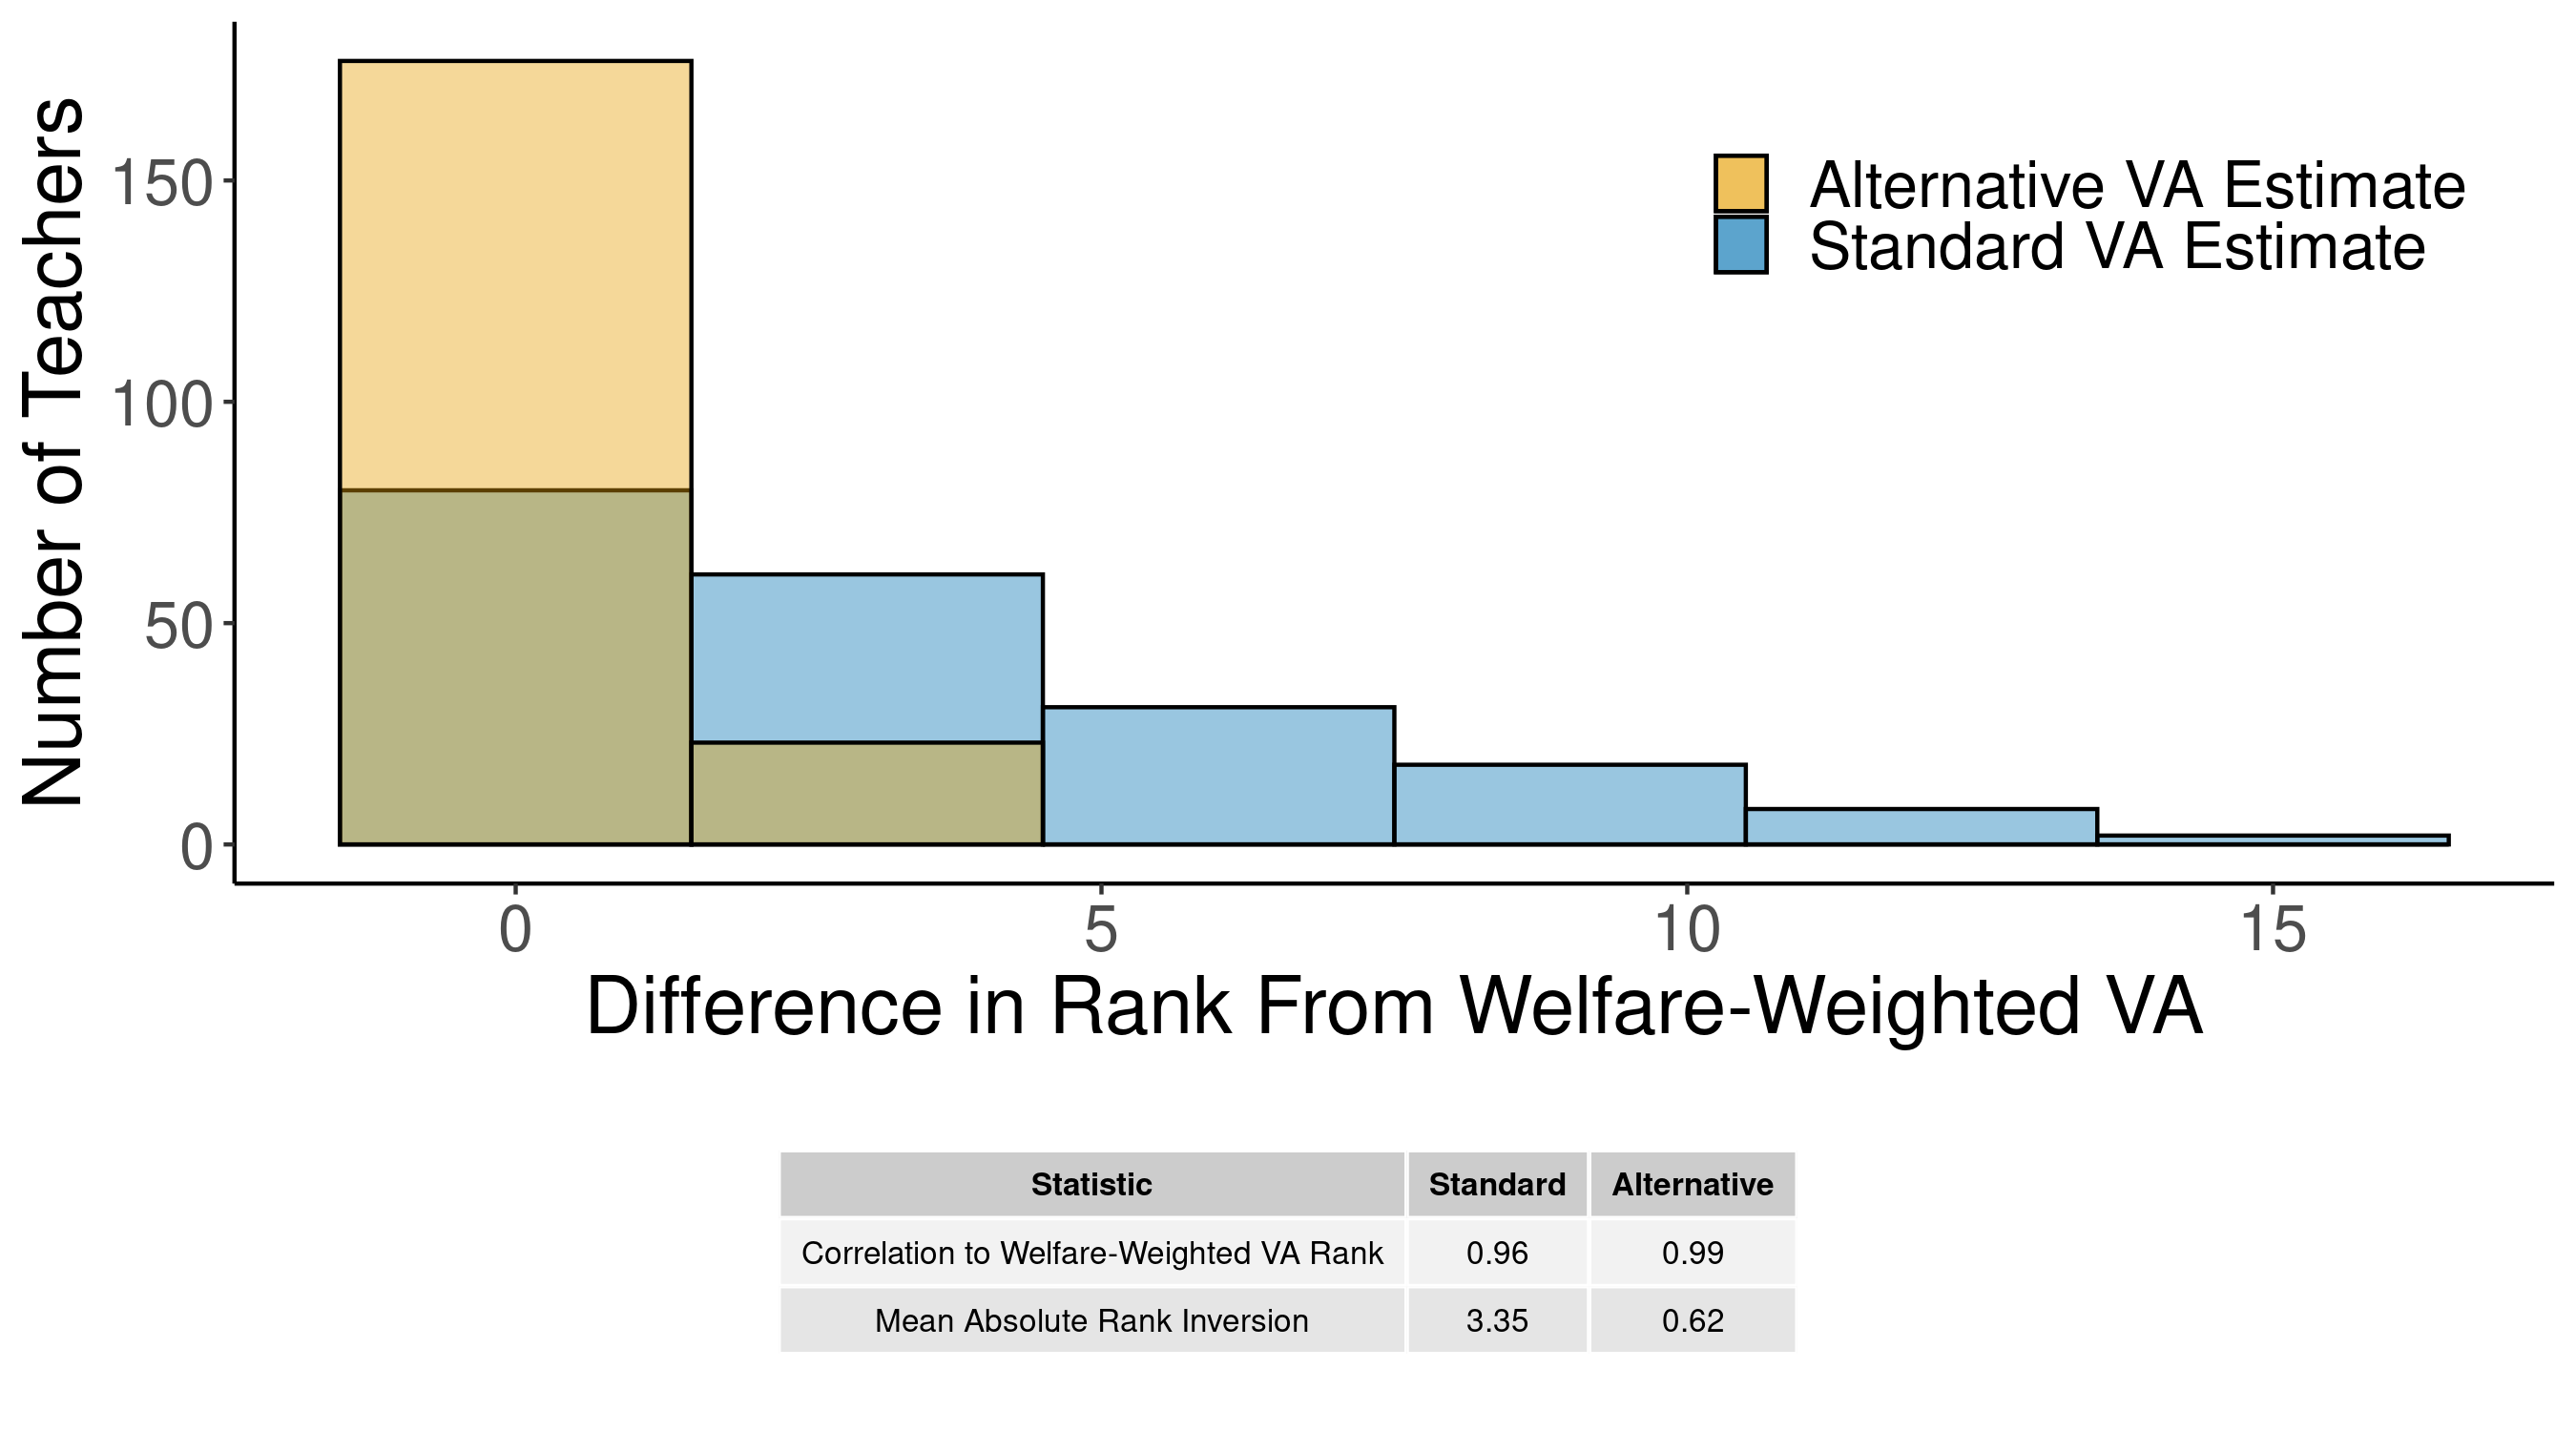
\includegraphics[width=\linewidth]{slides/Figures/np_hist_run_5.png}
        \end{subfigure}%
        \begin{subfigure}{.5\textwidth}
          \centering
          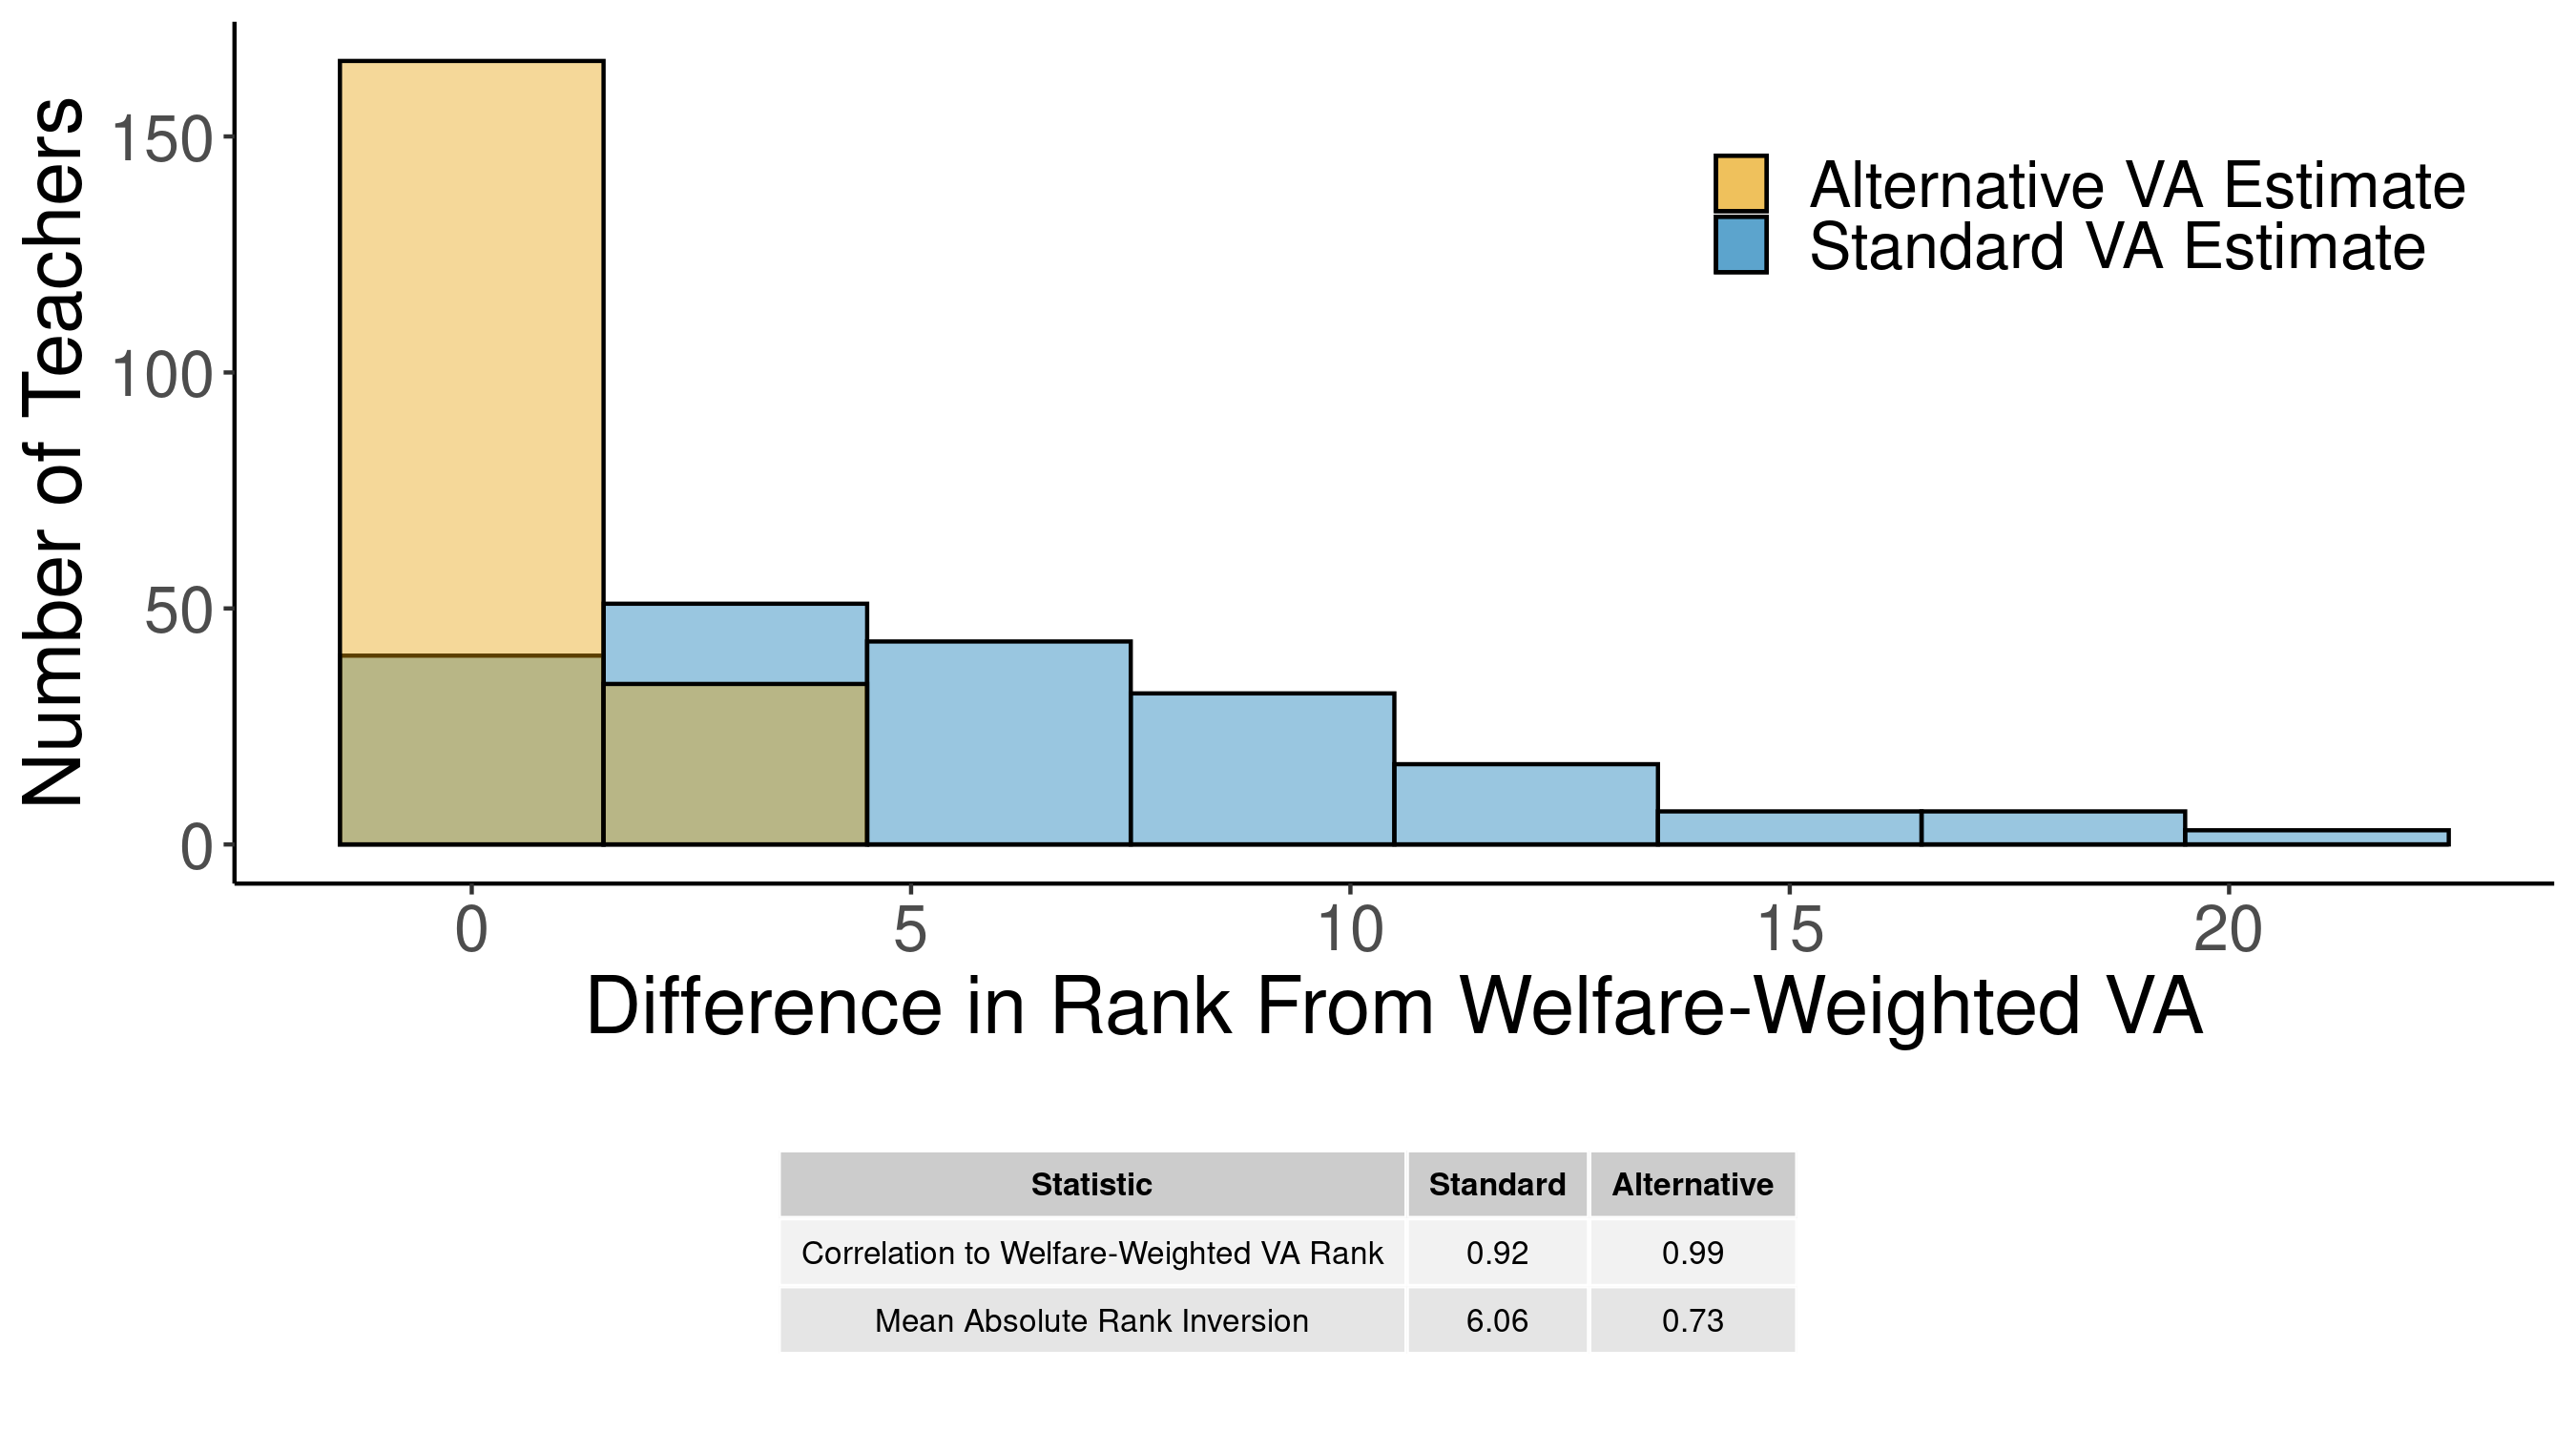
\includegraphics[width=\linewidth]{slides/Figures/np_hist_run_6.png}
        \end{subfigure}
        
        \begin{subfigure}{.5\textwidth}
          \centering
          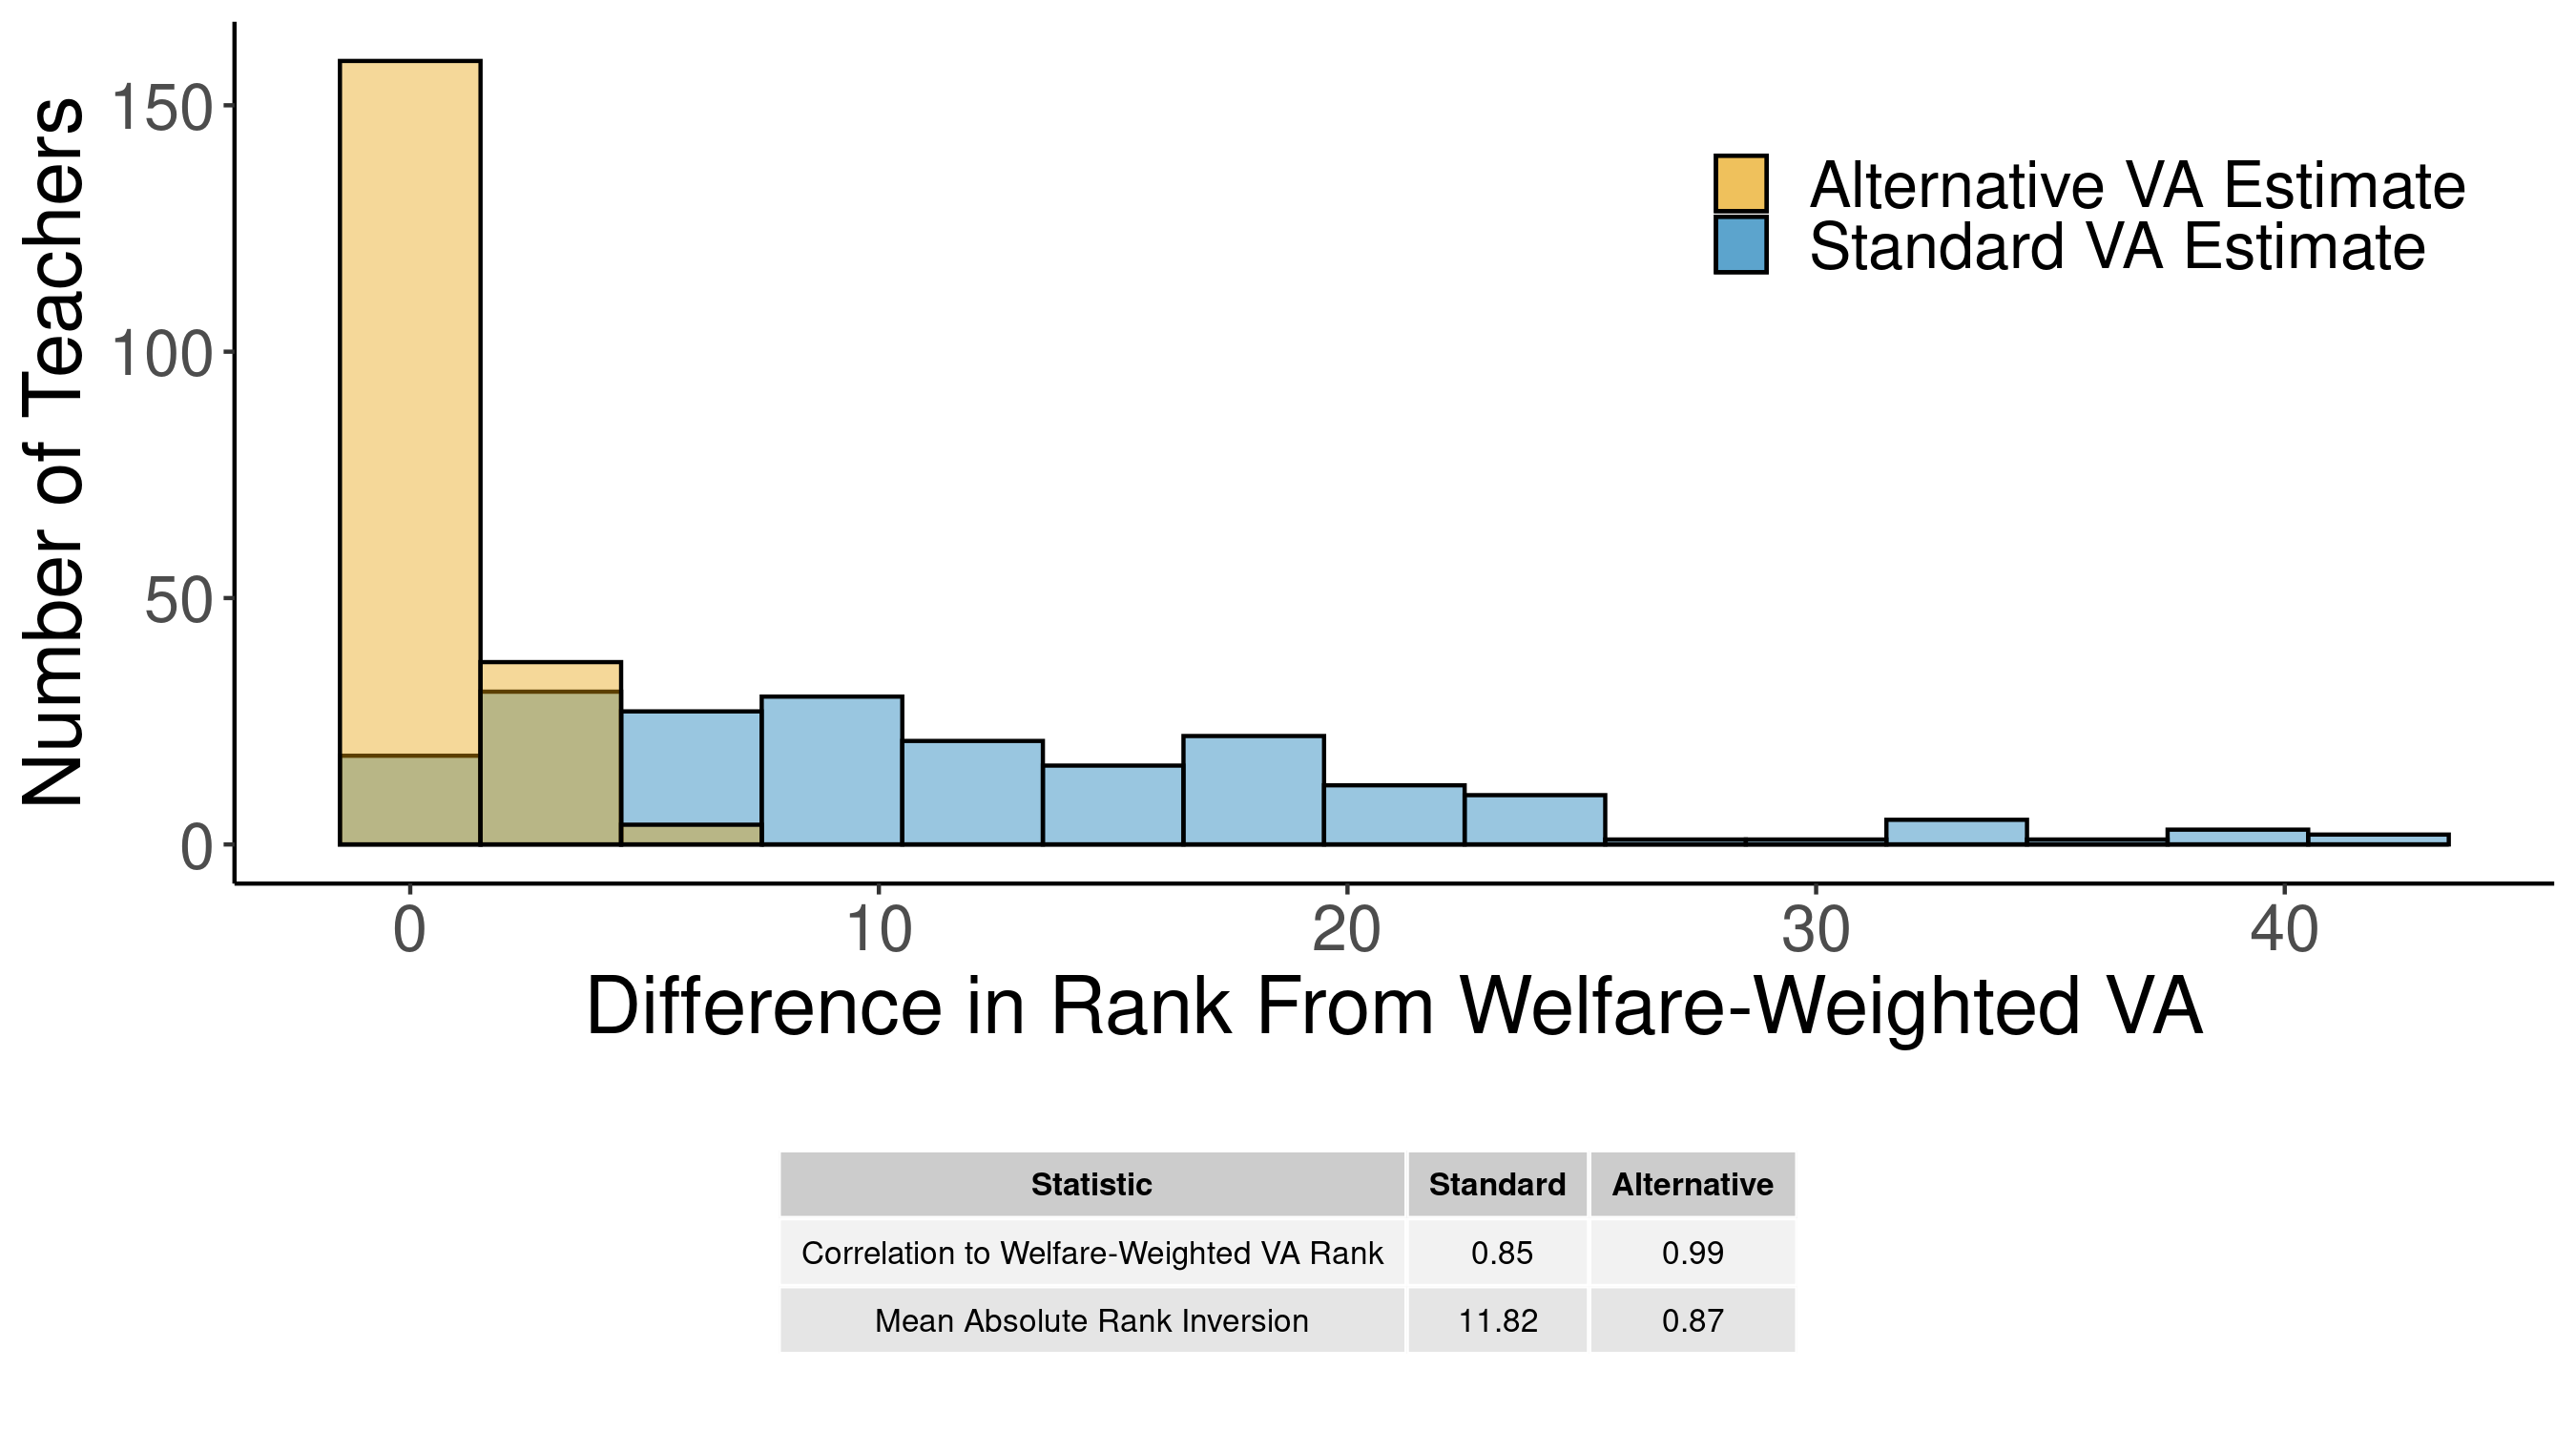
\includegraphics[width=\linewidth]{slides/Figures/np_hist_run_7.png}
        \end{subfigure}%
        \begin{subfigure}{.5\textwidth}
          \centering
          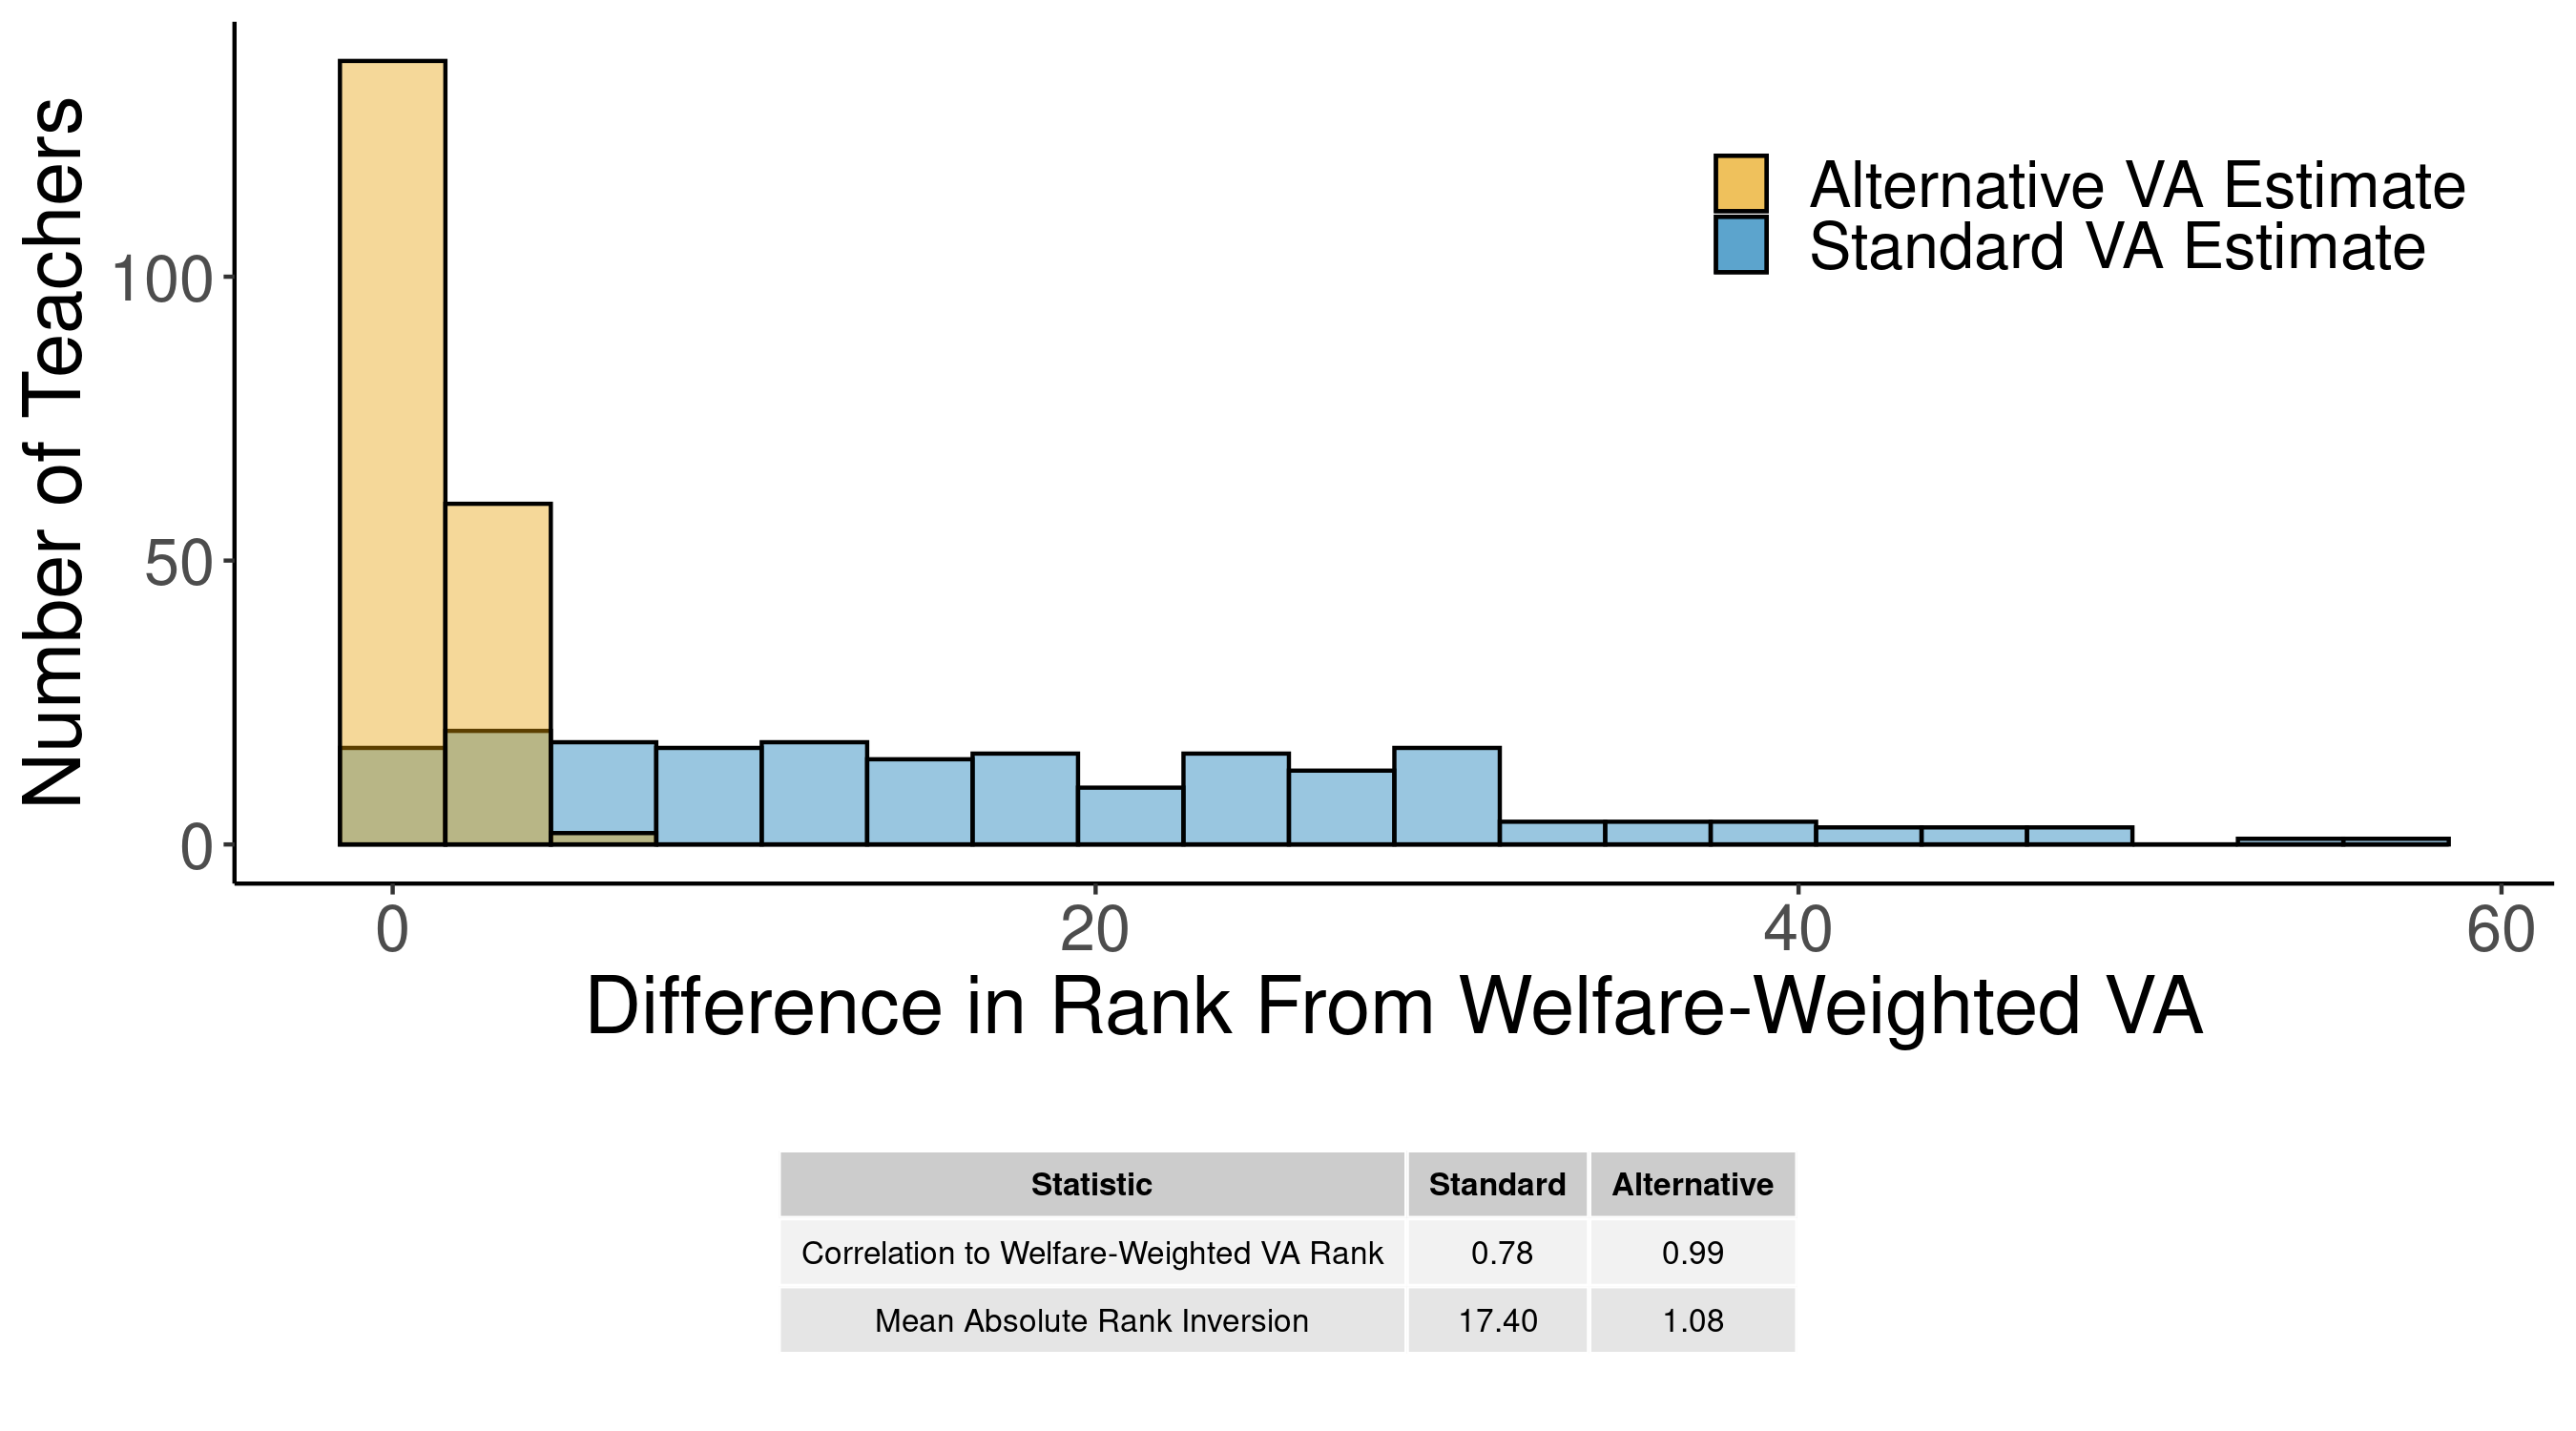
\includegraphics[width=\linewidth]{slides/Figures/np_hist_run_8.png}
        \end{subfigure}
    \end{figure}
    
    }
    
    %\only<2>{
    %\frametitle{Value of Teacher Ability Holding Match Quality Constant}
    %
    %\vfill
    %\begin{figure}
    %    \centering
    %    \begin{subfigure}{.5\textwidth}
    %      \centering
    %      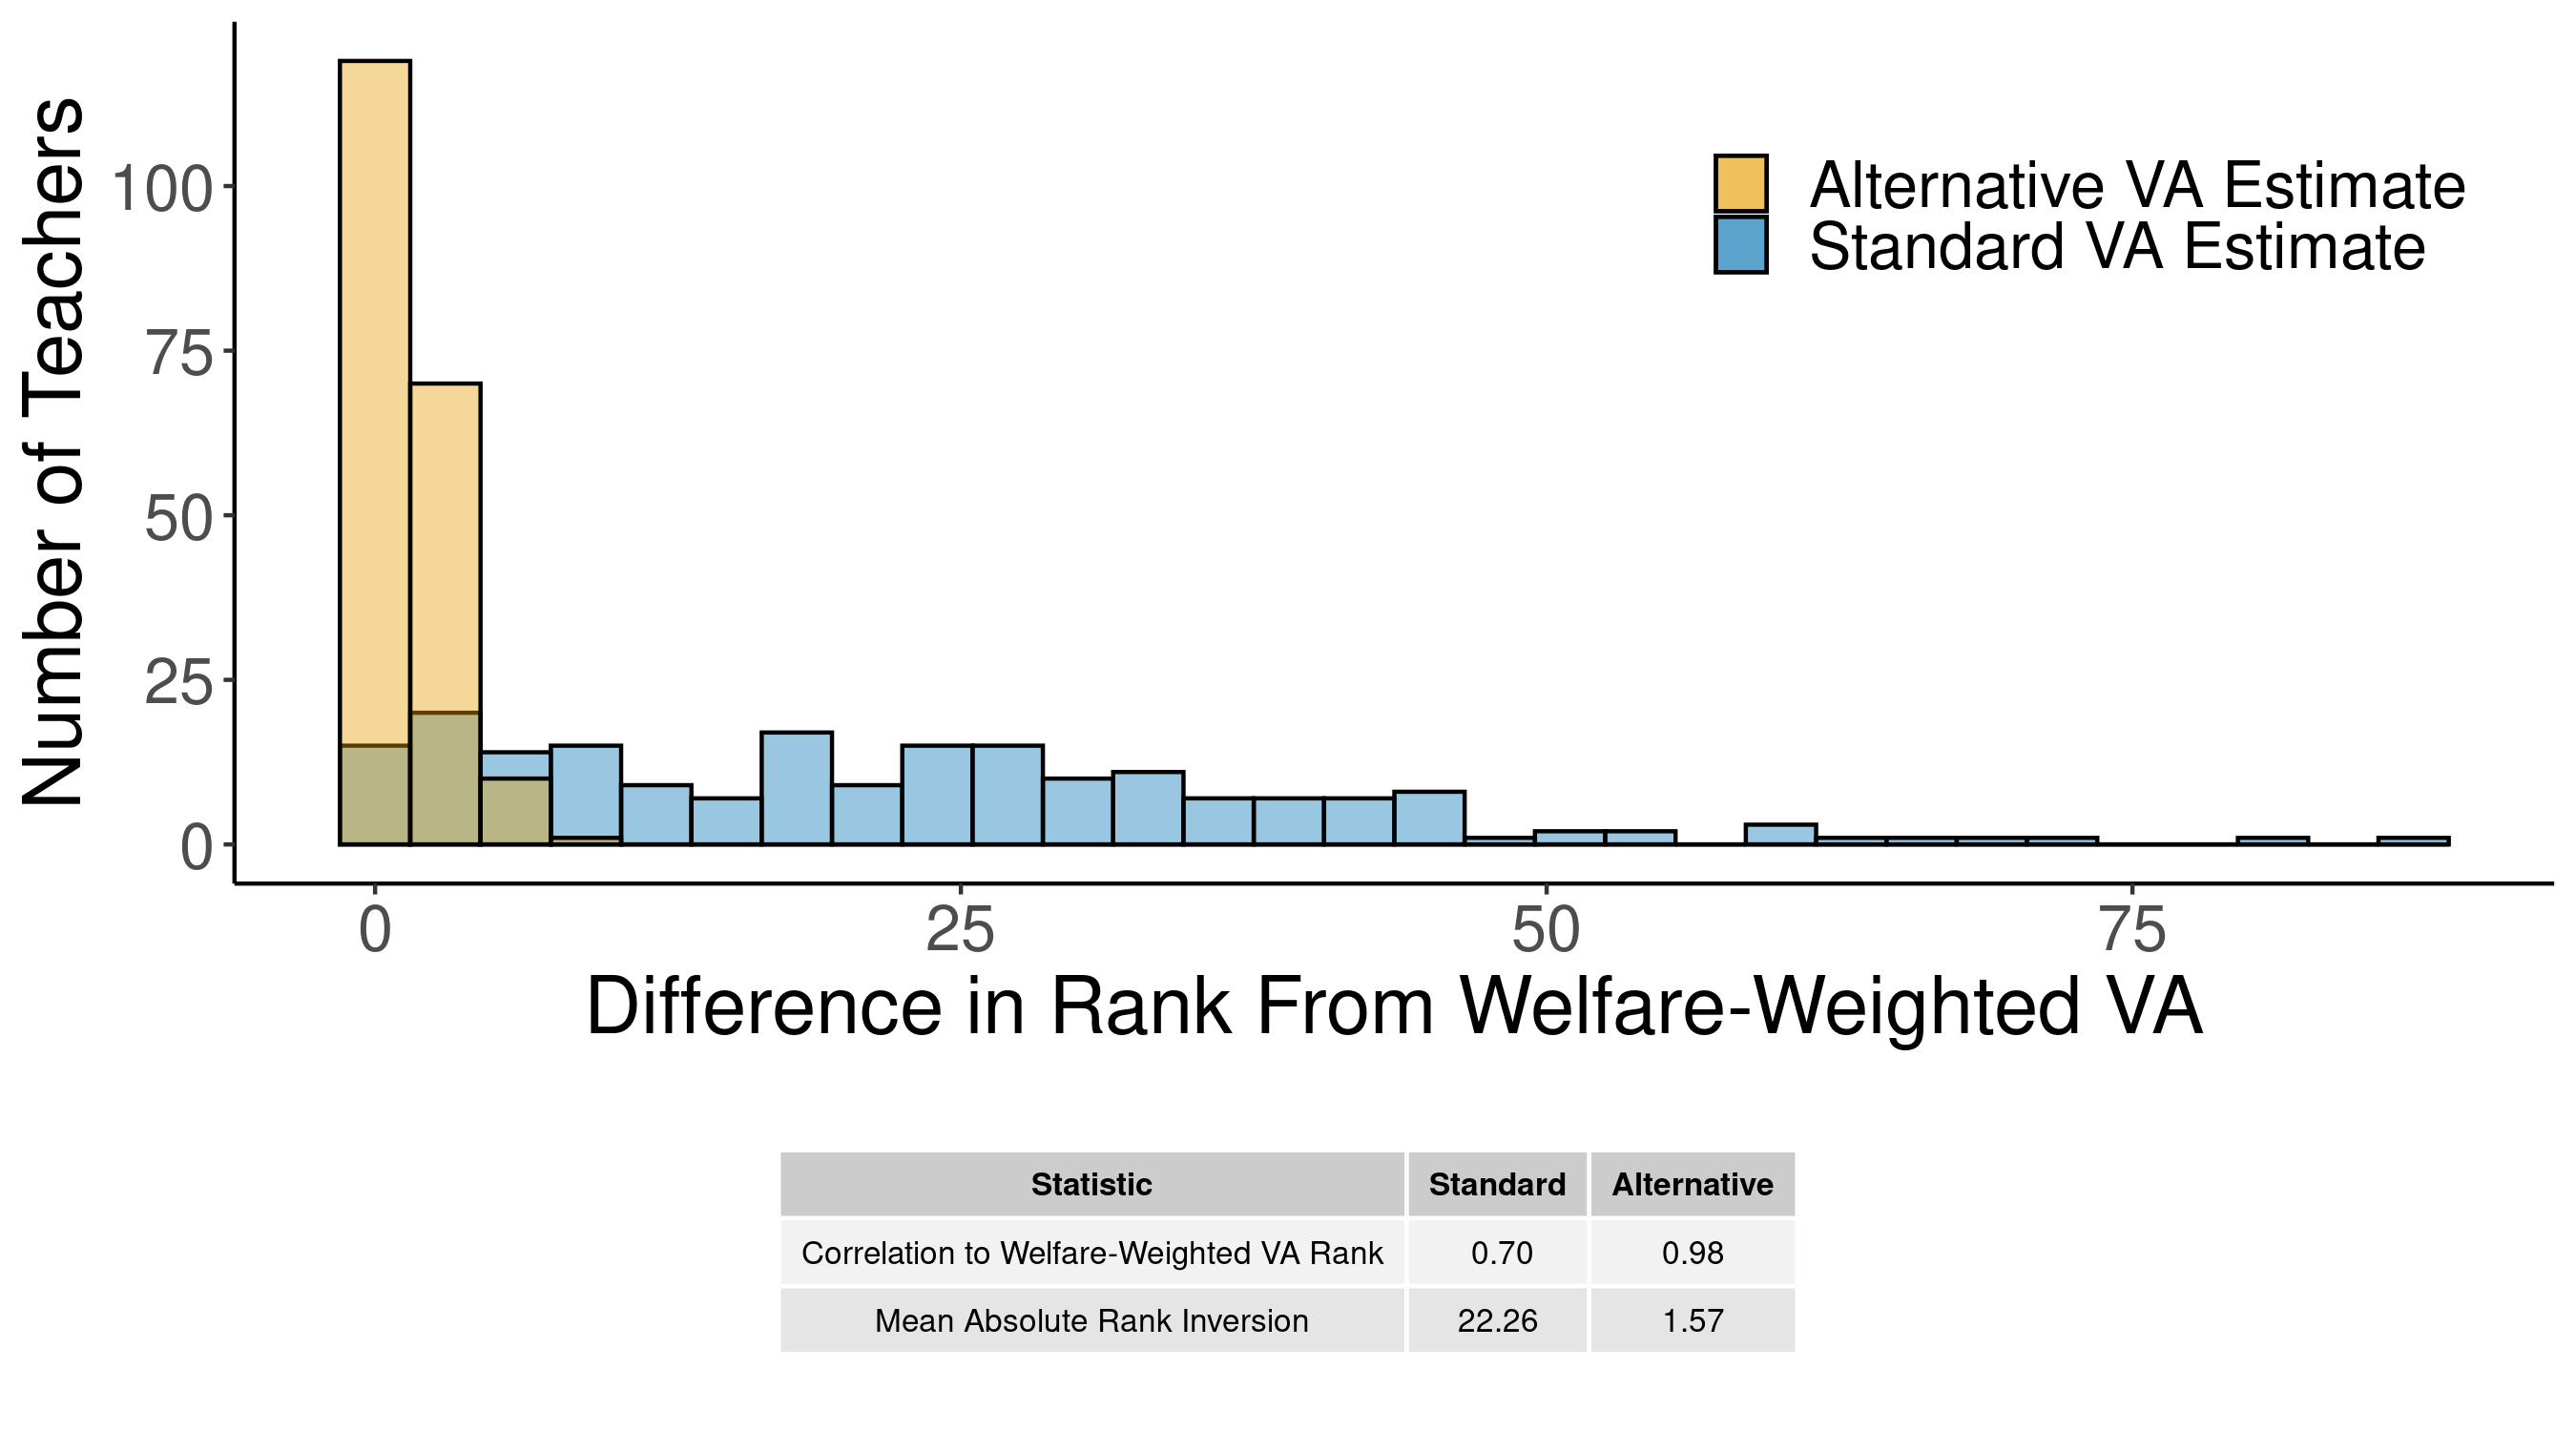
\includegraphics[width=\linewidth]{slides/Figures/np_hist_run_9.png}
    %    \end{subfigure}%
    %    \begin{subfigure}{.5\textwidth}
    %      \centering
    %      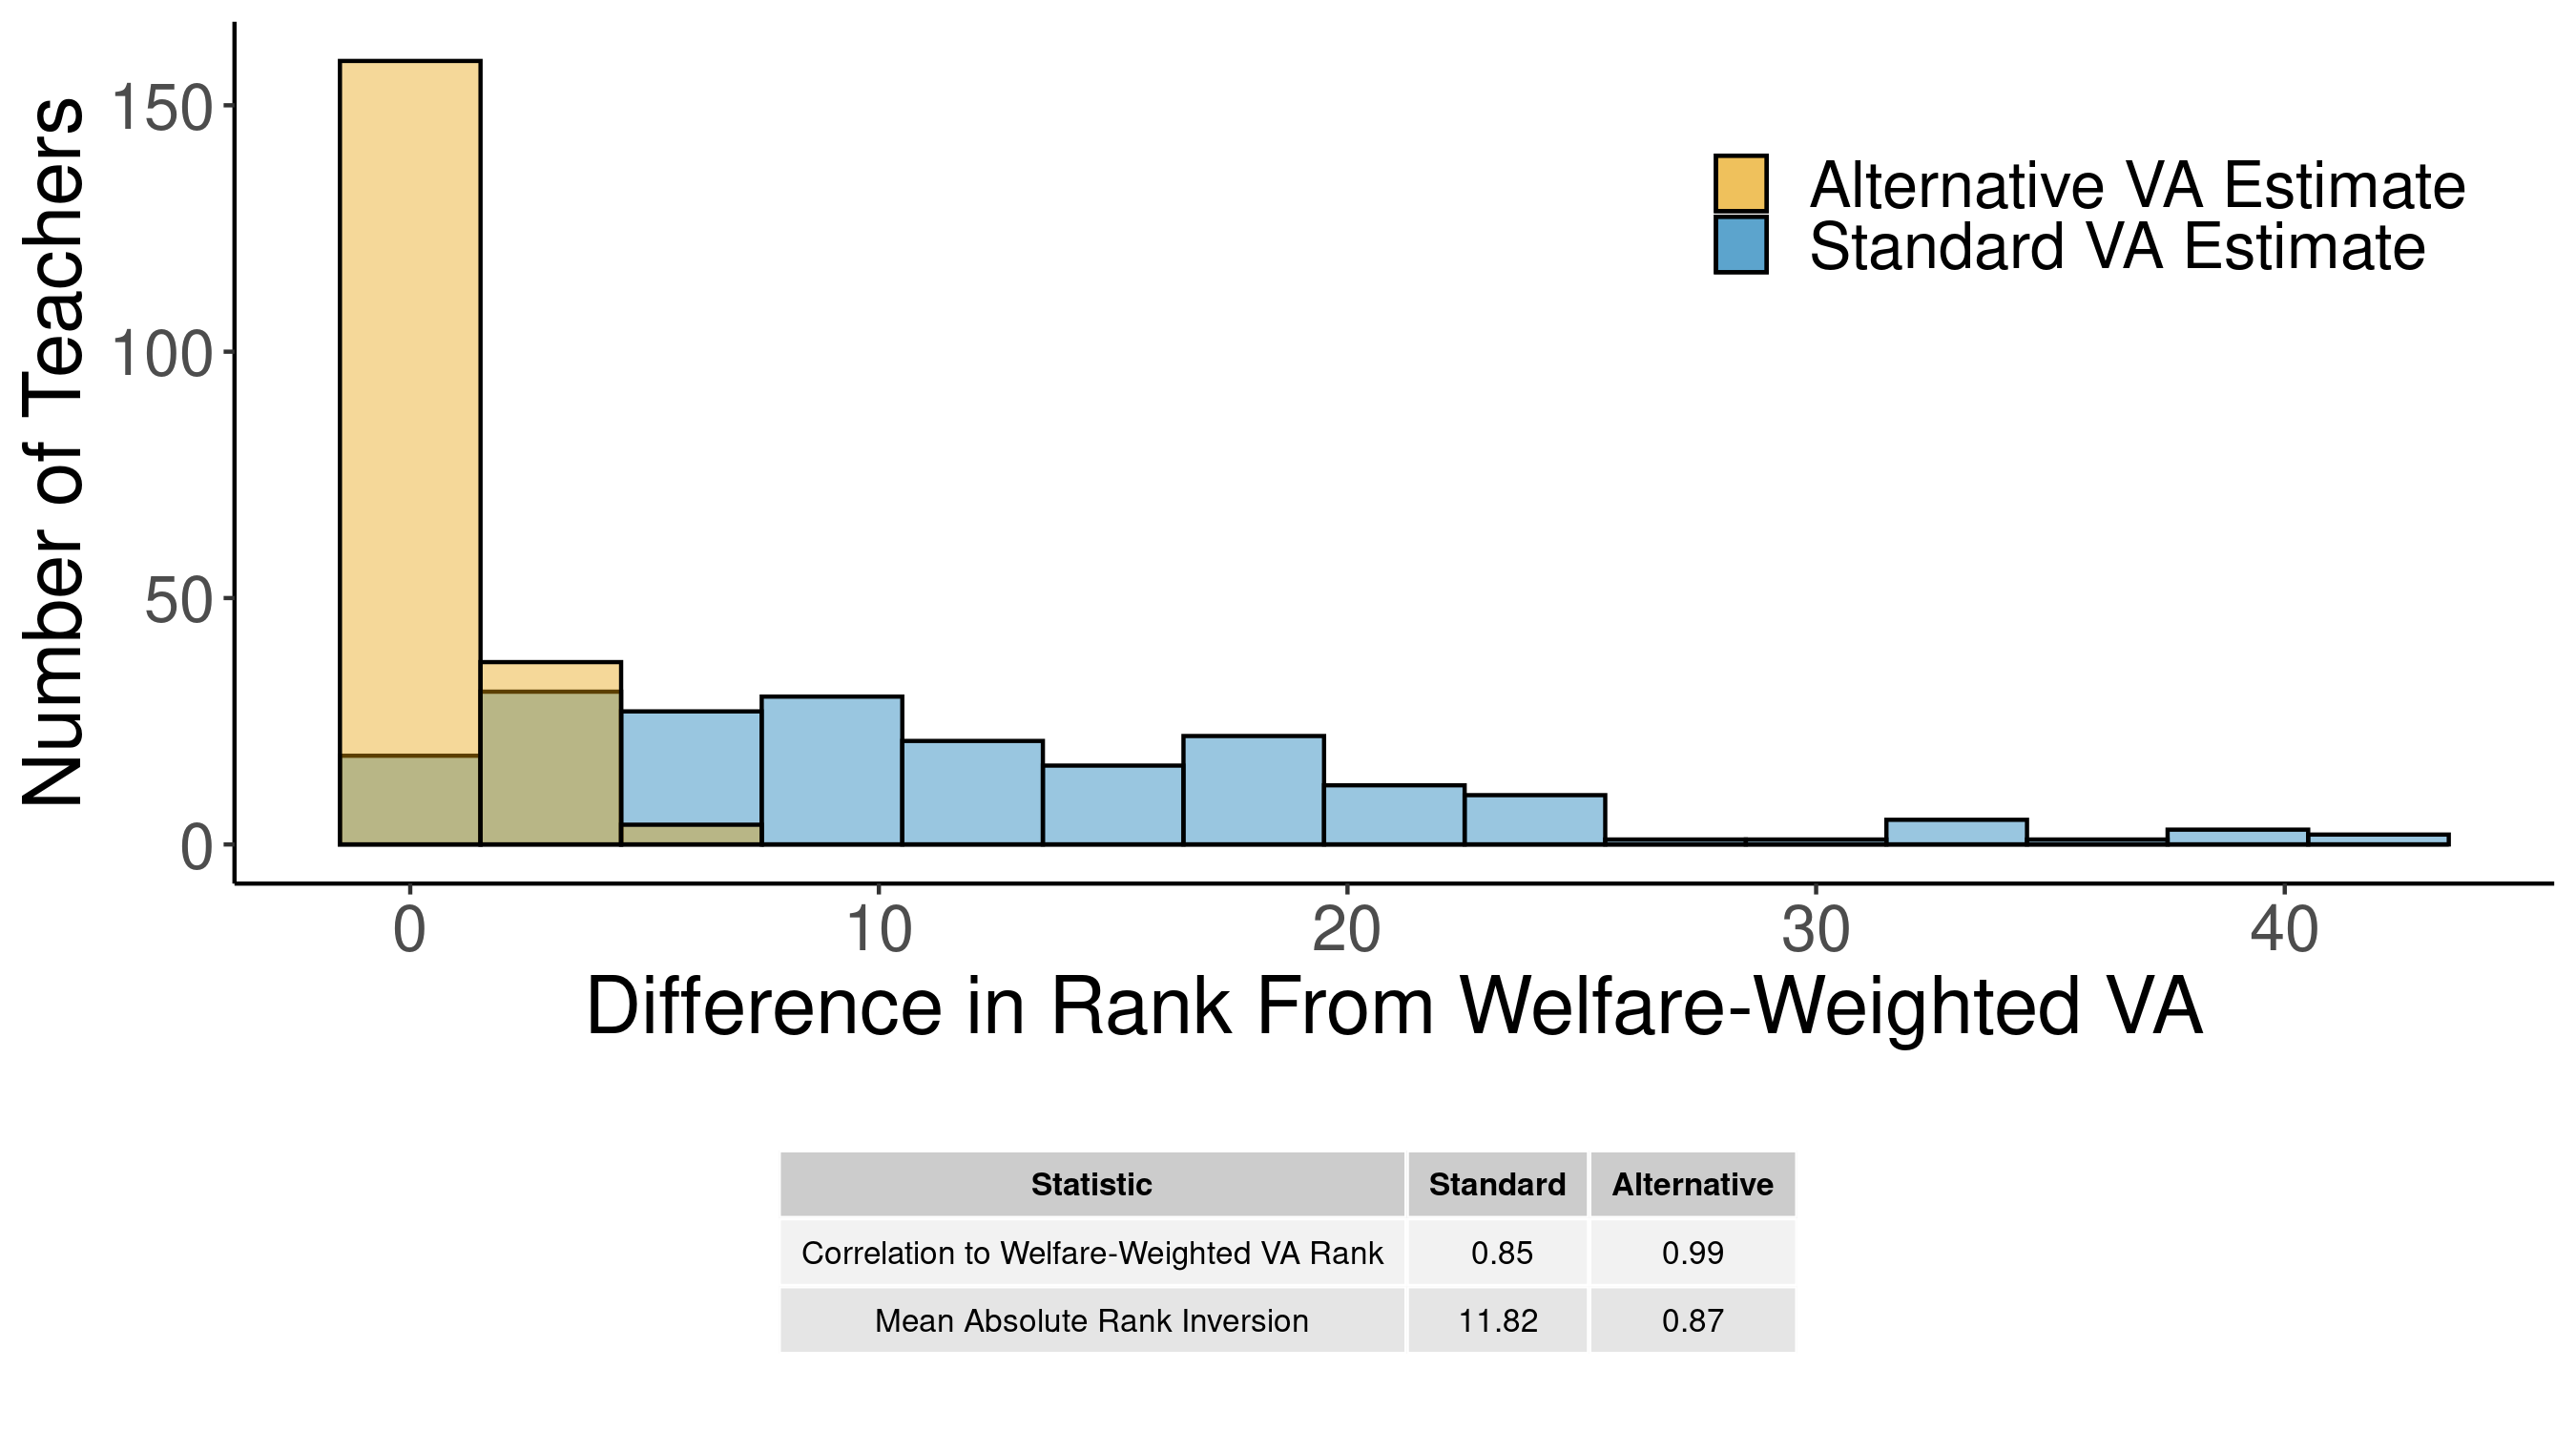
\includegraphics[width=\linewidth]{slides/Figures/np_hist_run_10.png}
    %    \end{subfigure}
    %    
    %    \begin{subfigure}{.5\textwidth}
    %      \centering
    %      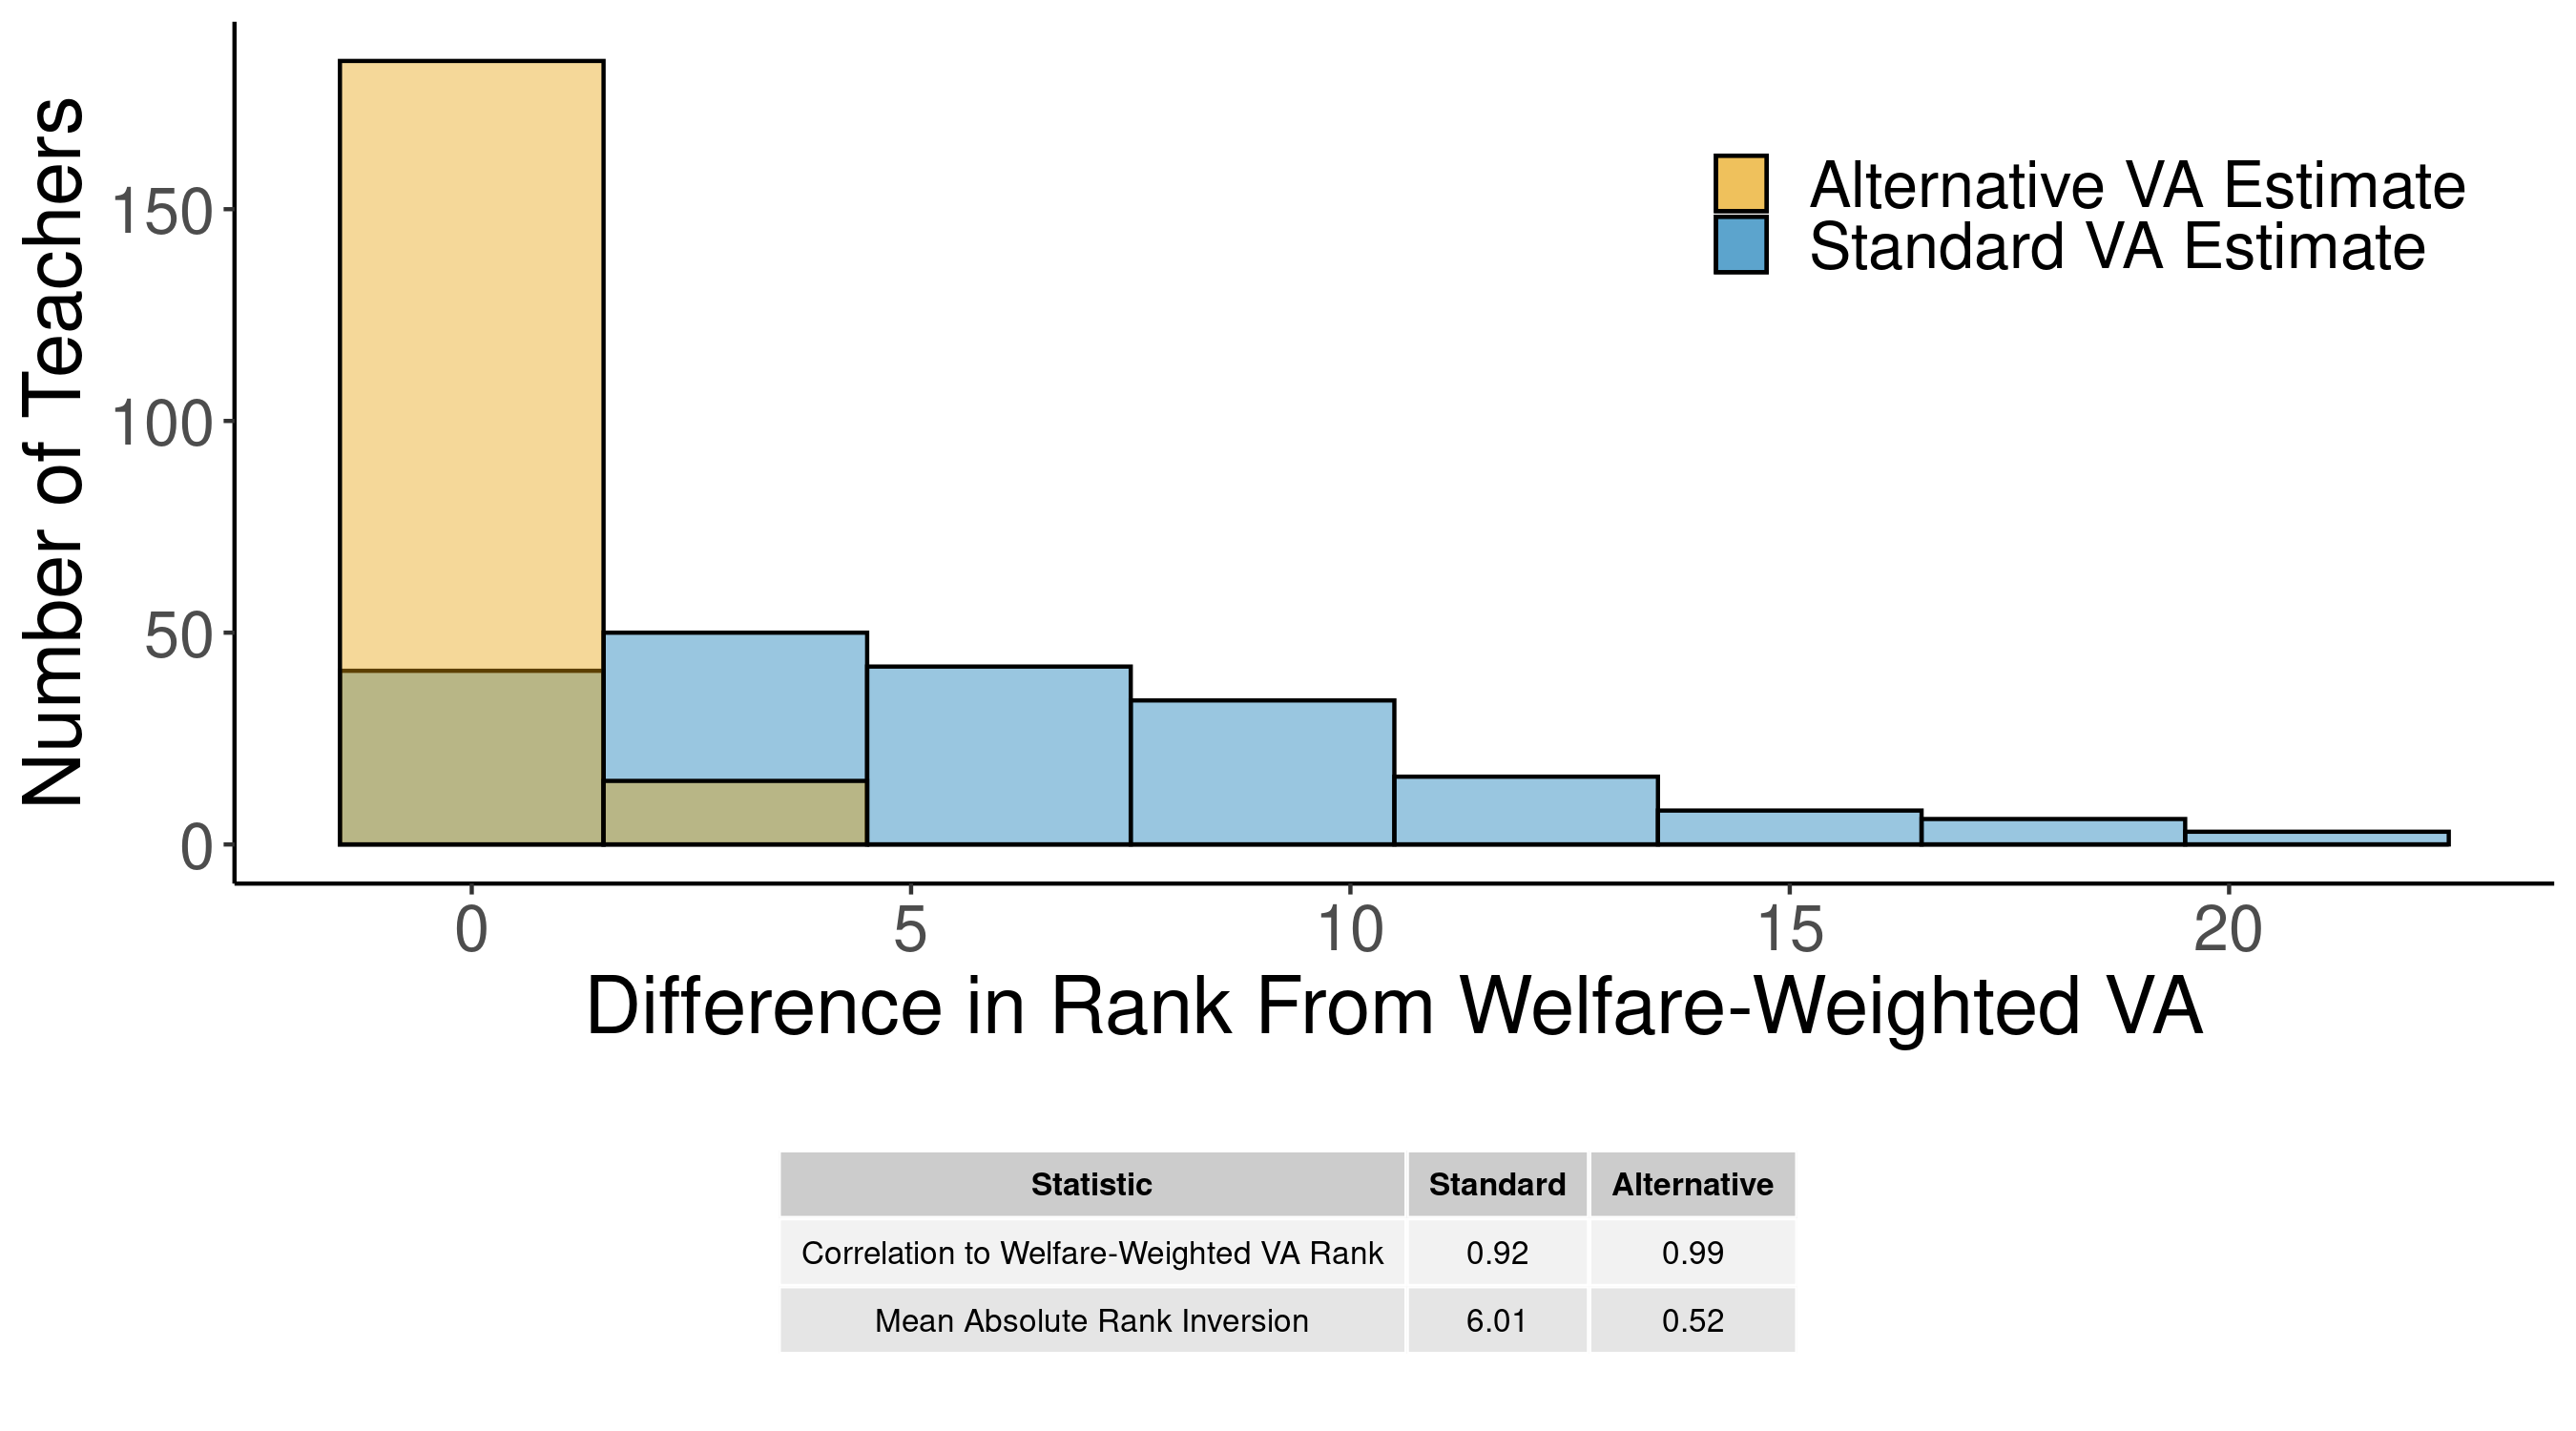
\includegraphics[width=\linewidth]{slides/Figures/np_hist_run_11.png}
    %    \end{subfigure}%
    %    \begin{subfigure}{.5\textwidth}
    %      \centering
    %      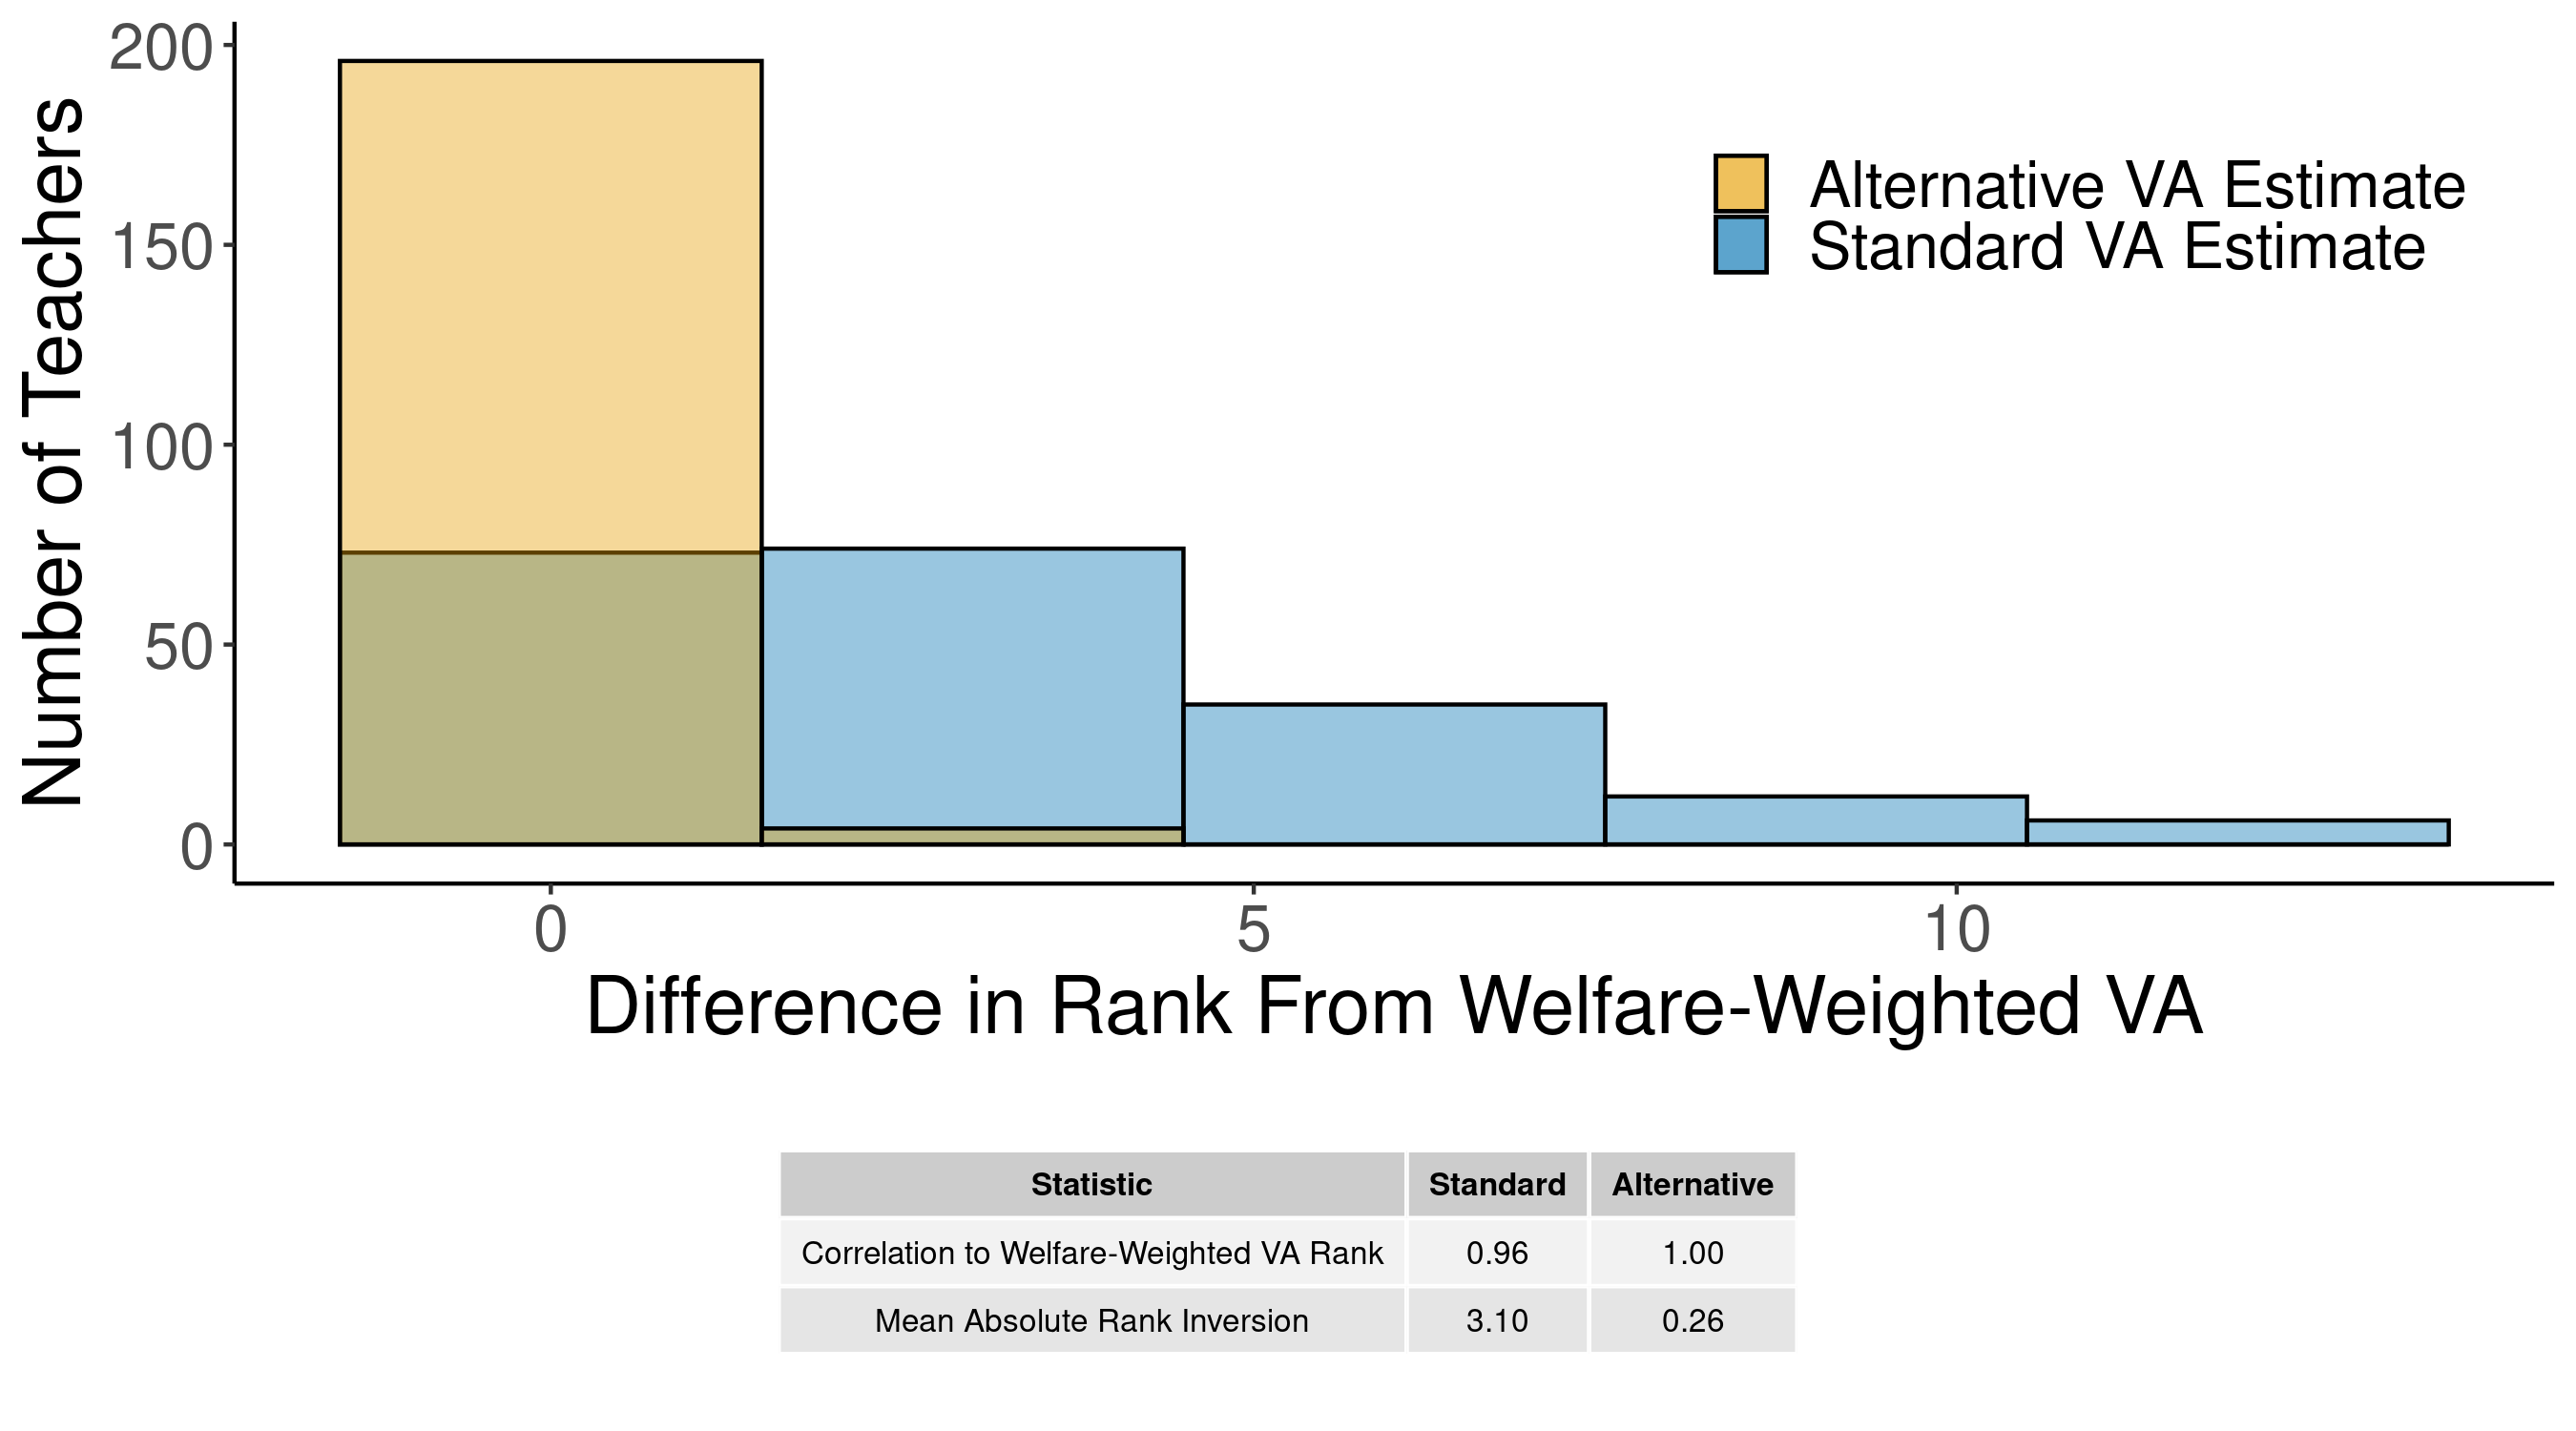
\includegraphics[width=\linewidth]{slides/Figures/np_hist_run_12.png}
    %    \end{subfigure}
    %\end{figure}
    %
    %}

\end{frame}


%%%%%%%%%%%%%%%%%%%%%%%%%%%%%%%%%%%%%%%%%%%%%%%%%%%%%%%%
%%%%%%%%%%%%%%%%%%%%%%%%%%%%%%%%%%%%%%%%%%%%%%%%%%%%%%%%

\begin{frame}{Including Student Sorting}

    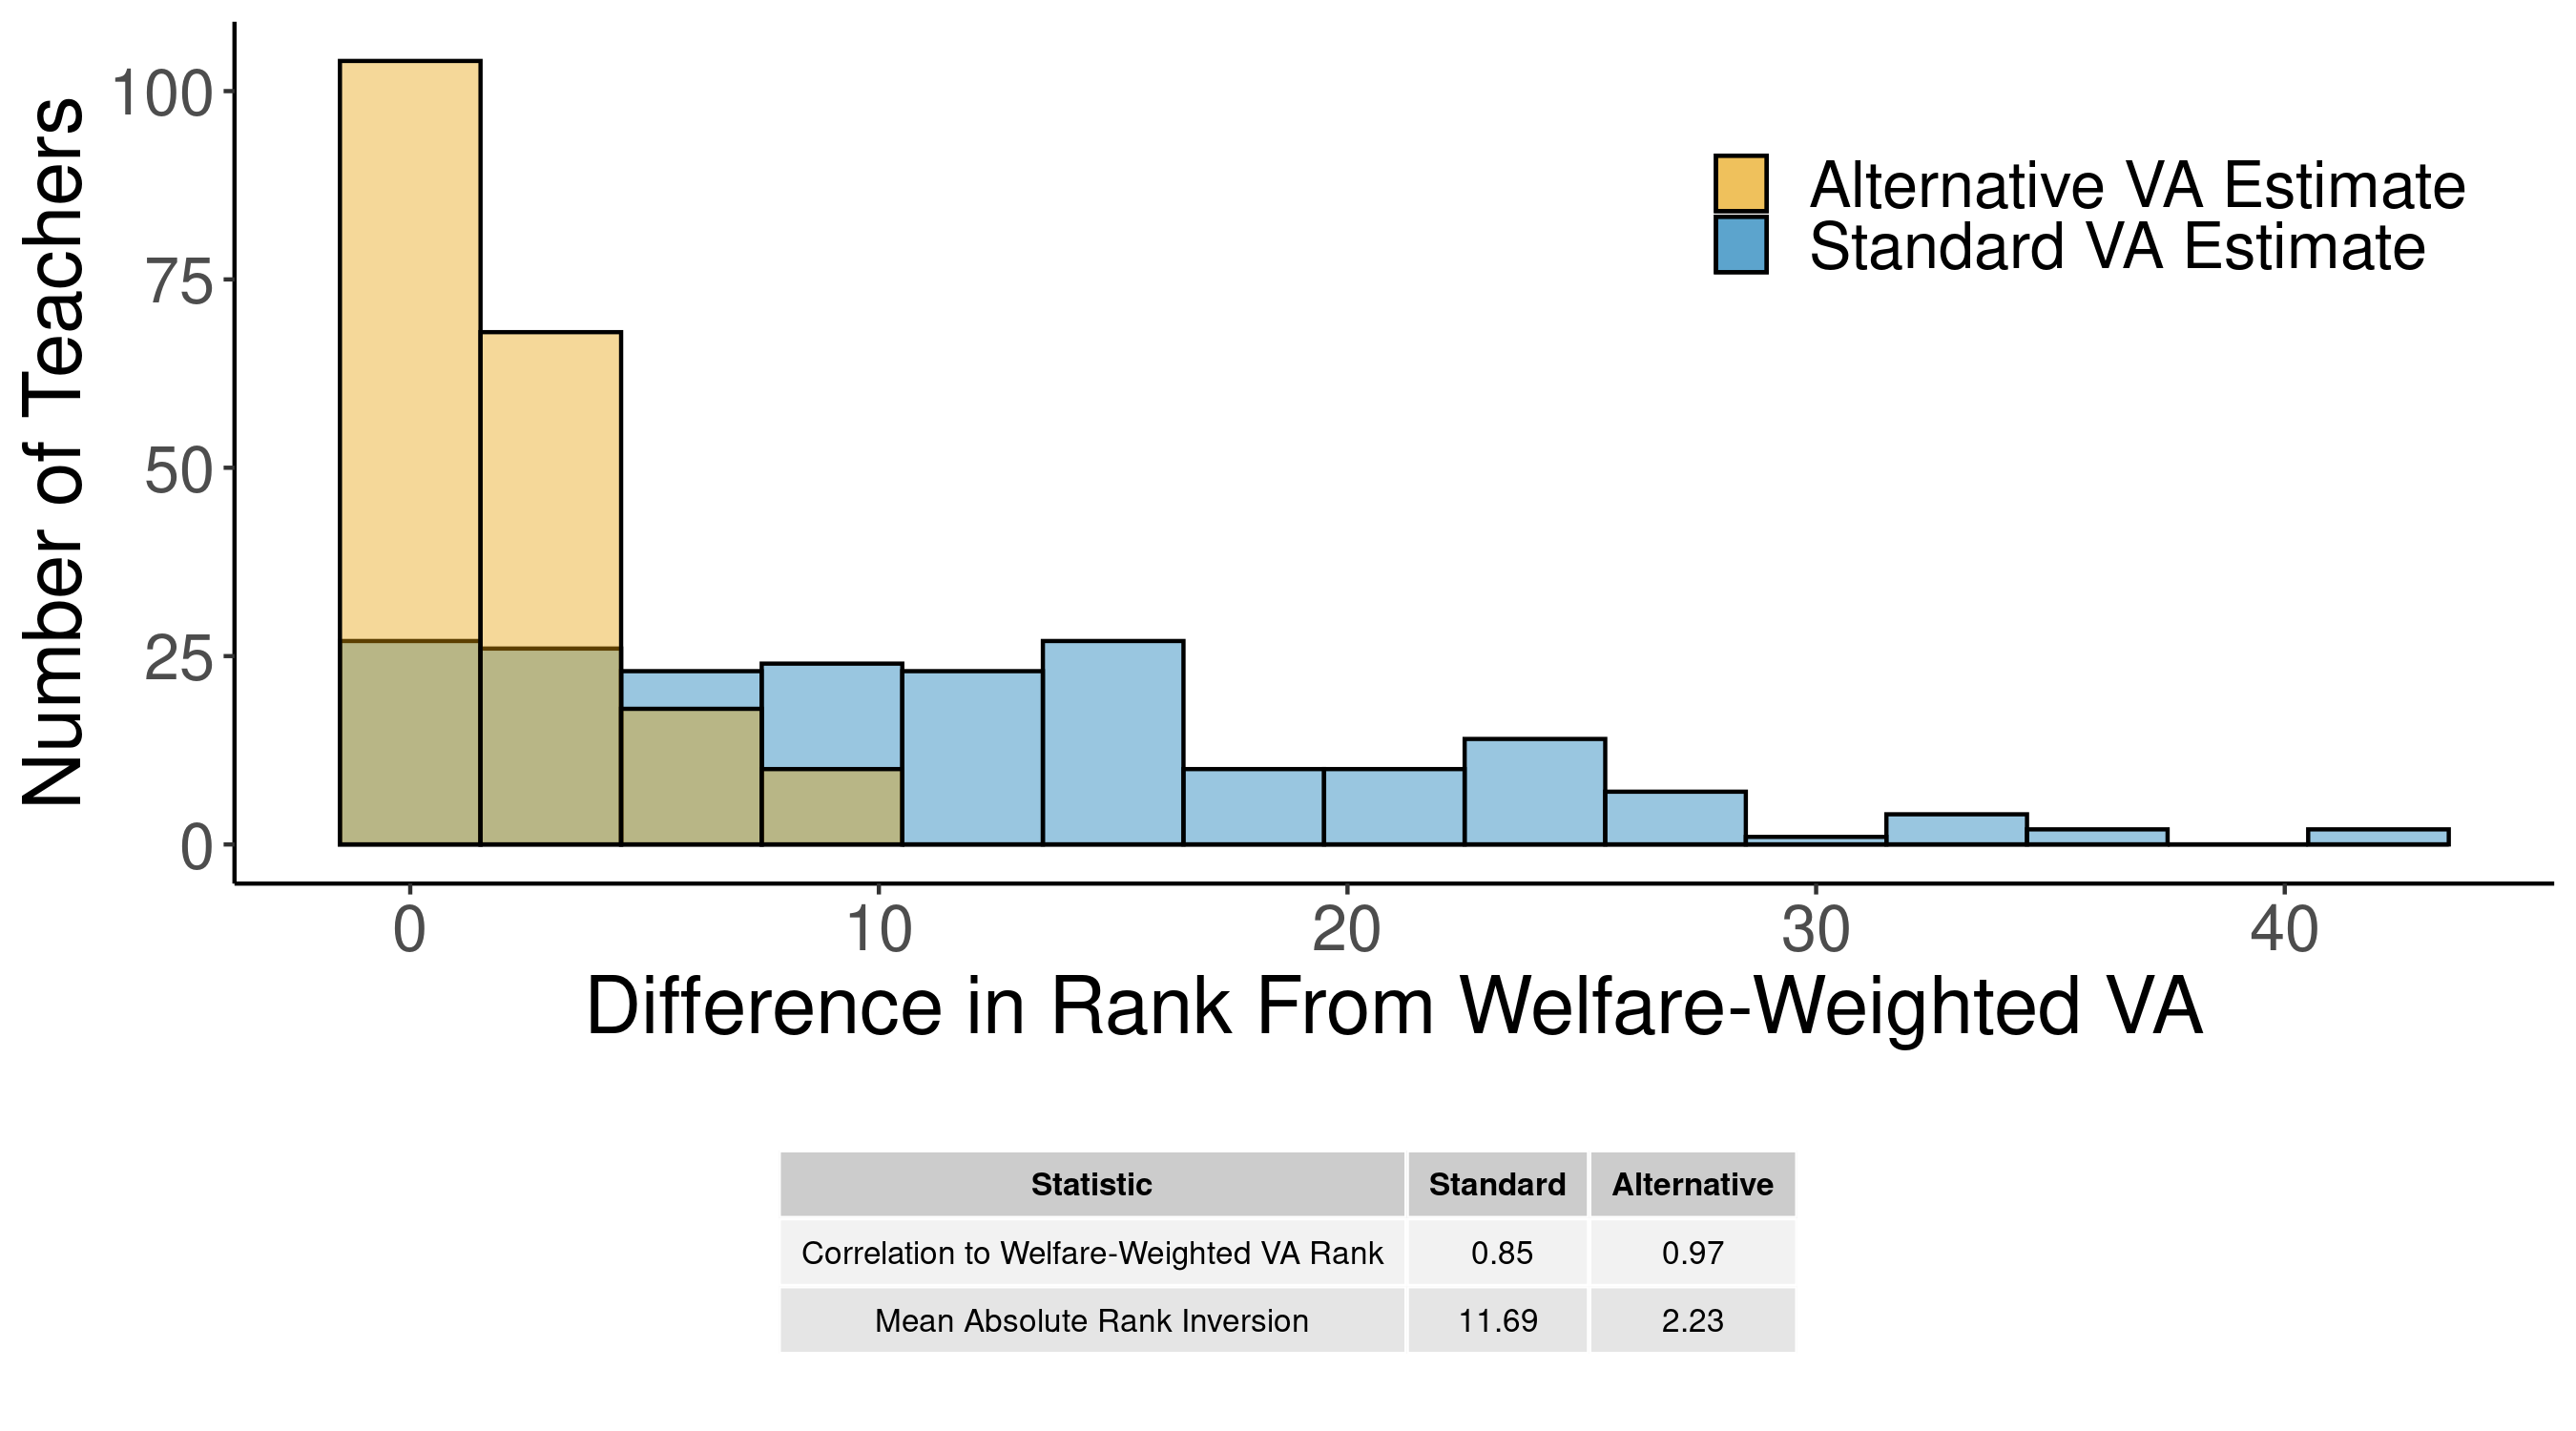
\includegraphics[width=\textwidth]{slides/Figures/np_hist_run_14.png}

\end{frame}


%%%%%%%%%%%%%%%%%%%%%%%%%%%%%%%%%%%%%%%%%%%%%%%%%%%%%%%%
%%%%%%%%%%%%%%%%%%%%%%%%%%%%%%%%%%%%%%%%%%%%%%%%%%%%%%%%

\begin{frame}{Including Student Sorting and Peer Effects}

    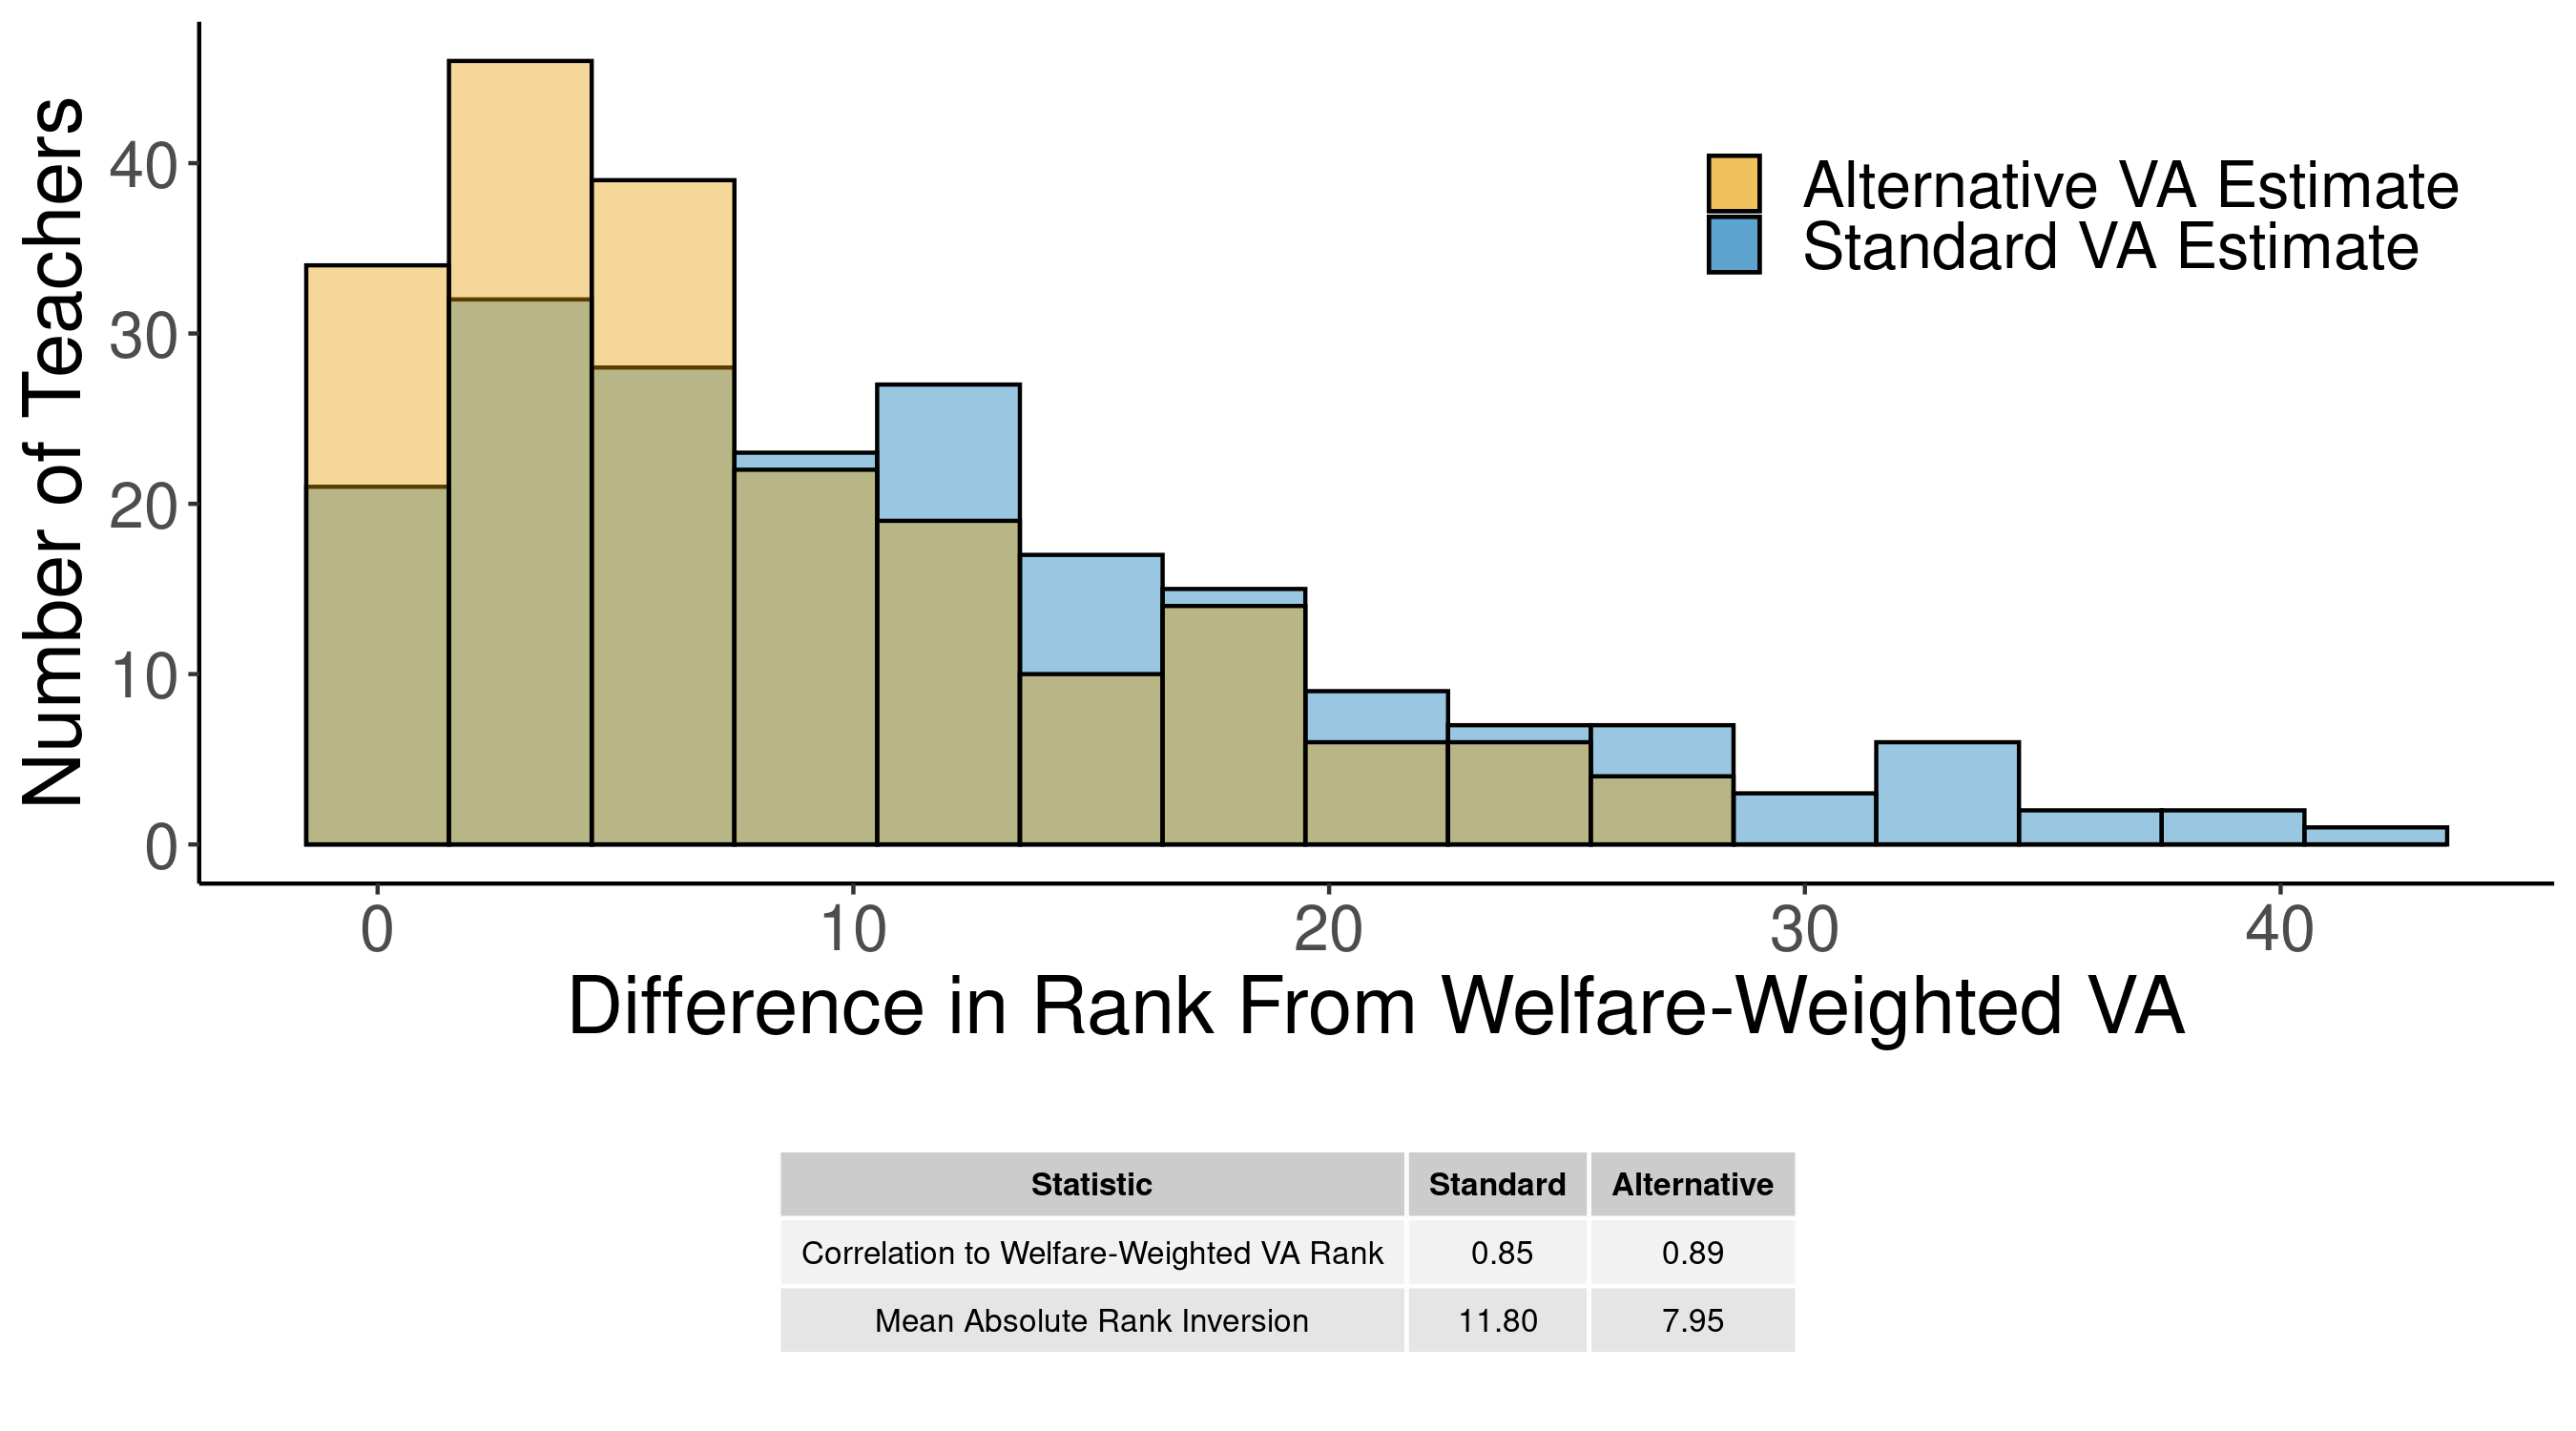
\includegraphics[width=\textwidth]{slides/Figures/np_hist_run_15.png}

\end{frame}





%%%%%%%%%%%%%%%%%%%%%%%%%%%%%%%%%%%%%%%%%%%%%%%%%%%%%%%%
%%%%%%%%%%%%%%%%% Empirical Application %%%%%%%%%%%%%%%%
%%%%%%%%%%%%%%%%%%%%%%%%%%%%%%%%%%%%%%%%%%%%%%%%%%%%%%%%

\section{Empirical Application}

%%%%%%%%%%%%%%%%%%%%%%%%%%%%%%%%%%%%%%%%%%%%%%%%%%%%%%%%
%%%%%%%%%%%%%%%%%%%%%%%%%%%%%%%%%%%%%%%%%%%%%%%%%%%%%%%%

\begin{frame}{What use is this in real data?}

    \begin{itemize}
        \item Construct an empirical test - how much does heterogeneity matter?
        \item Inform formal and informal tracking - how much could students benefit from being assigned to a teacher particularly suited to teaching them?
        \item Which teachers are especially successful at teaching target students? Administration may then be able to explore why those teachers are doing so well with target students and help to apply that more broadly.
    \end{itemize}
    
    We have initiated the process to acquire administrative data from a large school district to apply our methods and explore these questions.

\end{frame}


%%%%%%%%%%%%%%%%%%%%%%%%%%%%%%%%%%%%%%%%%%%%%%%%%%%%%%%%
%%%%%%%%%%%%%%%%%%%%%%%%%%%%%%%%%%%%%%%%%%%%%%%%%%%%%%%%

\begin{frame}{Possible Empirical Test}

    \only<1>{
    Idea - We compare the Kendall Rank Correlation Coefficient between the Standard VA Estimate and the Alternative VA Estimates. We also compare the Alternative VA Estimates to each other to evaluate whether we are just picking up noise.
    }
    
    \only<2>{
    \begin{table}
        \centering
        \caption*{Kendall Rank Correlation Between Estimated Rankings}
        \input{slides/Tables/Kendall.tex}
    \end{table}
    }

\end{frame}


%%%%%%%%%%%%%%%%%%%%%%%%%%%%%%%%%%%%%%%%%%%%%%%%%%%%%%%%
%%%%%%%%%%%%%%%%%%%%%%%%%%%%%%%%%%%%%%%%%%%%%%%%%%%%%%%%

\begin{frame}{Conclusion and Next Steps}

    
    This work suggests that heterogeneity in match quality across the achievement distribution could have important implications for use of traditional VAM in identifying highly effective teachers when policymakers target specific subgroups of students.

    \begin{itemize}
        \item Explore simulations further, stress test parameter choices and primitives
        \item Get data to better calibrate our simulations, apply our methods, and explore welfare implications
        \item Possible extensions like teacher effort or policy incentives rather than just ability
    \end{itemize}

\end{frame}


%%%%%%%%%%%%%%%%%%%%%%%%%%%%%%%%%%%%%%%%%%%%%%%%%%%%%%%%
%%%%%%%%%%%%%%%%%%%%%%%%%%%%%%%%%%%%%%%%%%%%%%%%%%%%%%%%

\begin{frame}{}

    \centering
    \Huge Thank you!

\end{frame}






%%%%%%%%%%%%%%%%%%%%%%%%%%%%%%%%%%%%%%%%%%%%%%%%%%%%%%%%
%%%%%%%%%%%%%%%%%%%%%% References %%%%%%%%%%%%%%%%%%%%%%
%%%%%%%%%%%%%%%%%%%%%%%%%%%%%%%%%%%%%%%%%%%%%%%%%%%%%%%%

\section*{}

%%%%%%%%%%%%%%%%%%%%%%%%%%%%%%%%%%%%%%%%%%%%%%%%%%%%%%%%
%%%%%%%%%%%%%%%%%%%%%%%%%%%%%%%%%%%%%%%%%%%%%%%%%%%%%%%%

\begin{frame}[noframenumbering, shrink=10]
    \frametitle{References}
    \bibliography{citations}
\end{frame}




%%%%%%%%%%%%%%%%%%%%%%%%%%%%%%%%%%%%%%%%%%%%%%%%%%%%%%%%
%%%%%%%%%%%%%%%%%%%%%%% Appendix %%%%%%%%%%%%%%%%%%%%%%%
%%%%%%%%%%%%%%%%%%%%%%%%%%%%%%%%%%%%%%%%%%%%%%%%%%%%%%%%


%%%%%%%%%%%%%%%%%%%%%%%%%%%%%%%%%%%%%%%%%%%%%%%%%%%%%%%%
%%%%%%%%%%%%%%%%%%%%%%%%%%%%%%%%%%%%%%%%%%%%%%%%%%%%%%%%

\section*{}
\begin{frame}[noframenumbering]{Only Variation in Teacher Ability}

\hypertarget{st_cent1}{}
\vfill

\begin{figure}
    \centering
 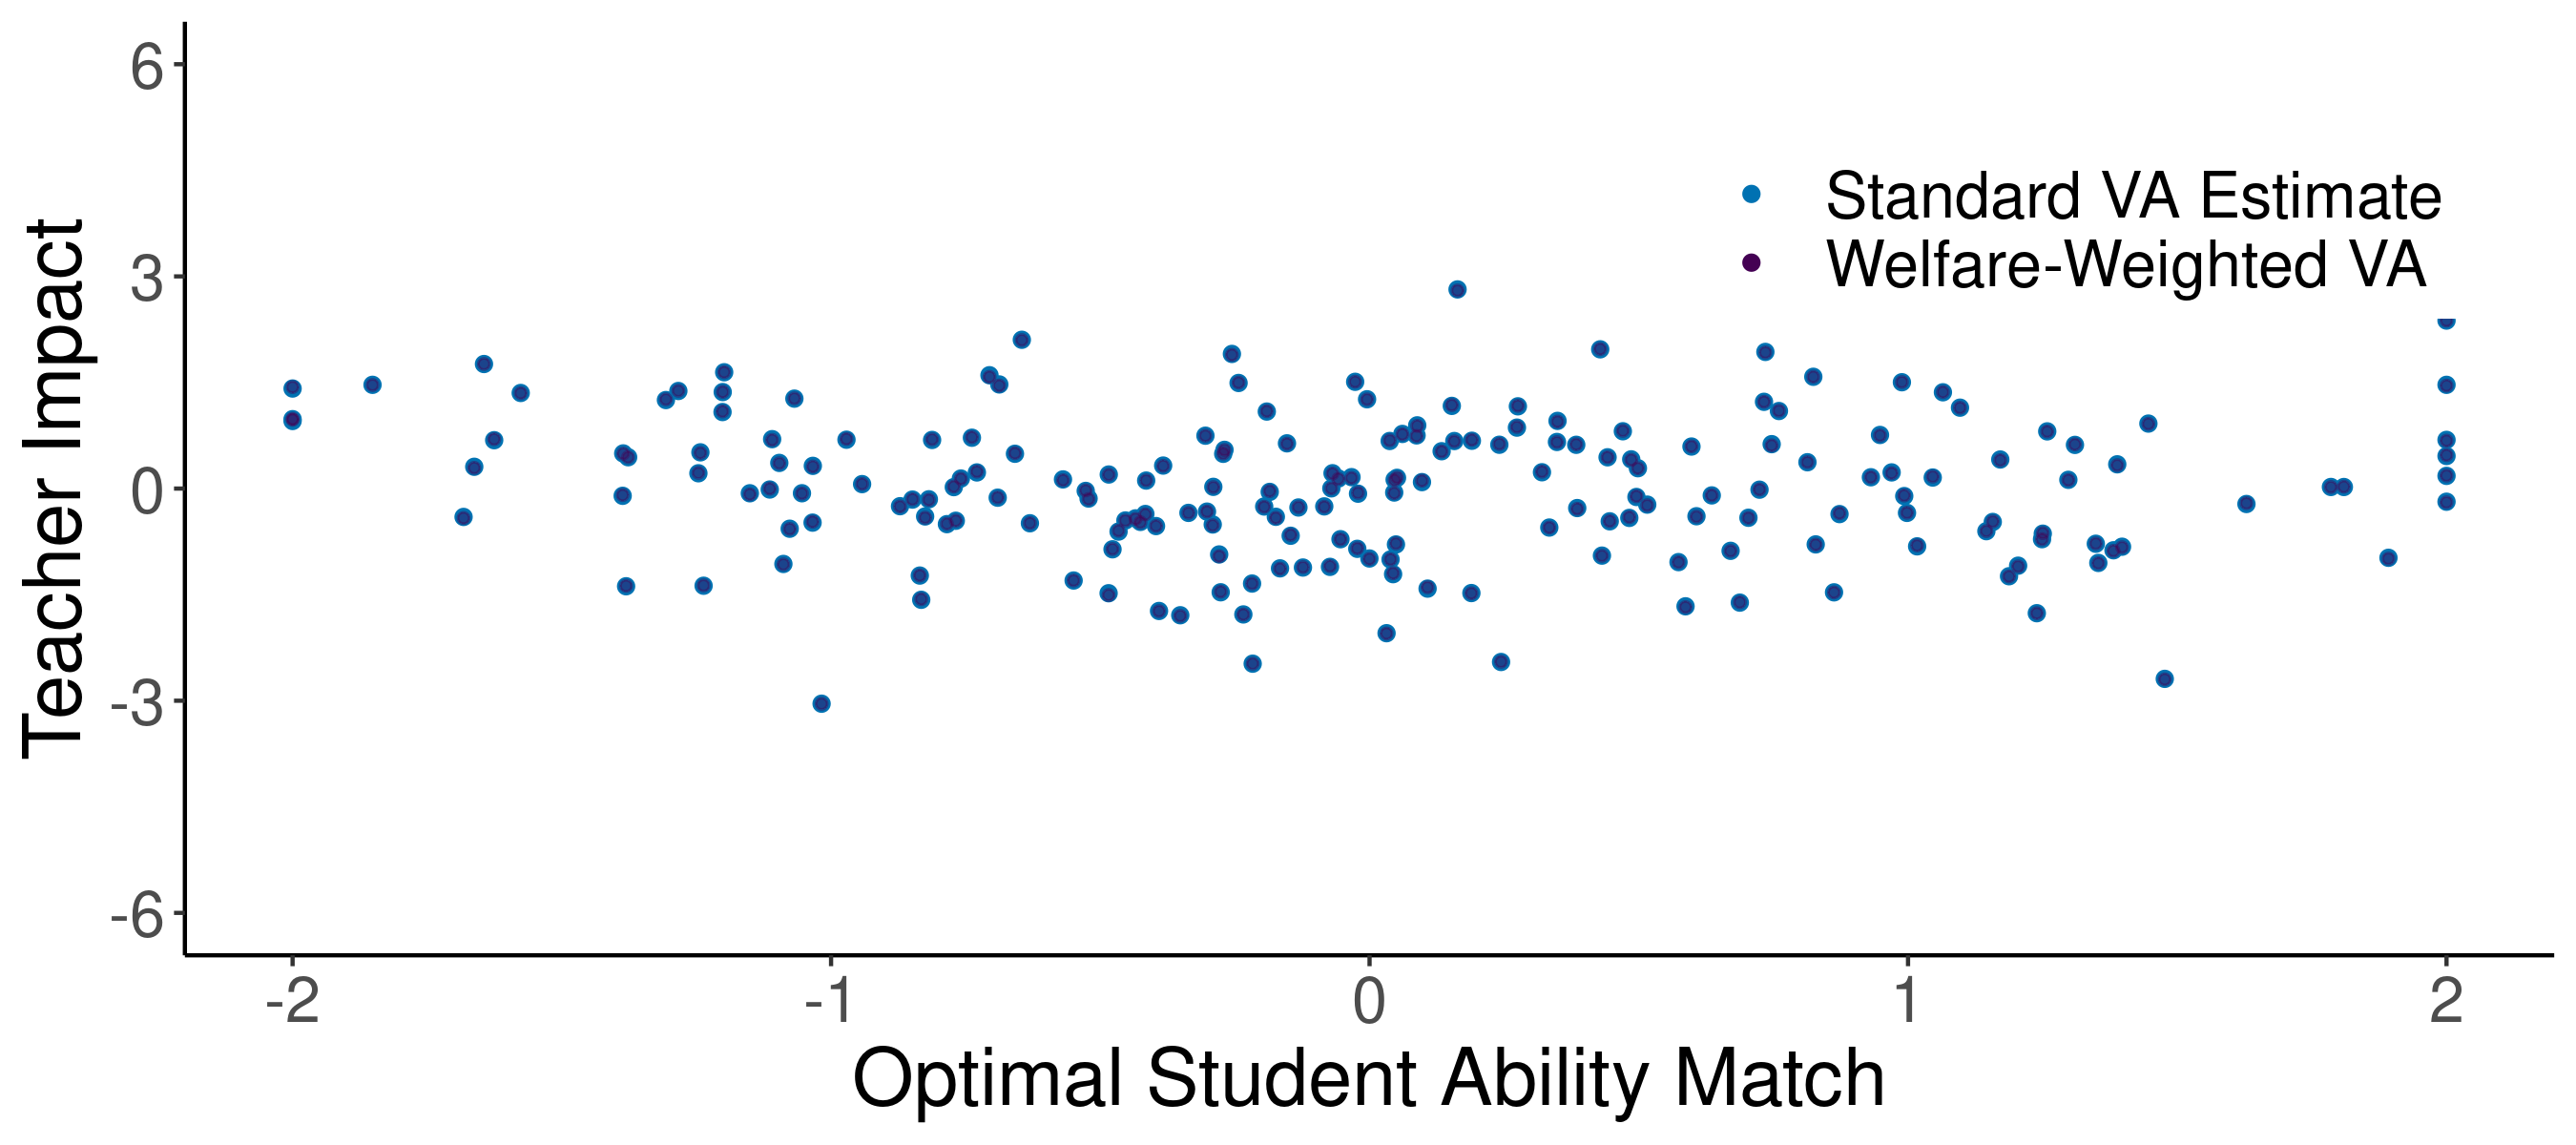
\includegraphics[width=.75\textwidth]{slides/Figures/standard_est_cent_run_1.png}
\end{figure}

\hyperlink{teacher_ability1}{\beamerbutton{Back}}

\end{frame}


%%%%%%%%%%%%%%%%%%%%%%%%%%%%%%%%%%%%%%%%%%%%%%%%%%%%%%%%
%%%%%%%%%%%%%%%%%%%%%%%%%%%%%%%%%%%%%%%%%%%%%%%%%%%%%%%%

\section*{}
\begin{frame}[noframenumbering]{Only Variation in Teacher Ability}

\hypertarget{np_cent1}{}
\vfill

\begin{figure}
    \centering
 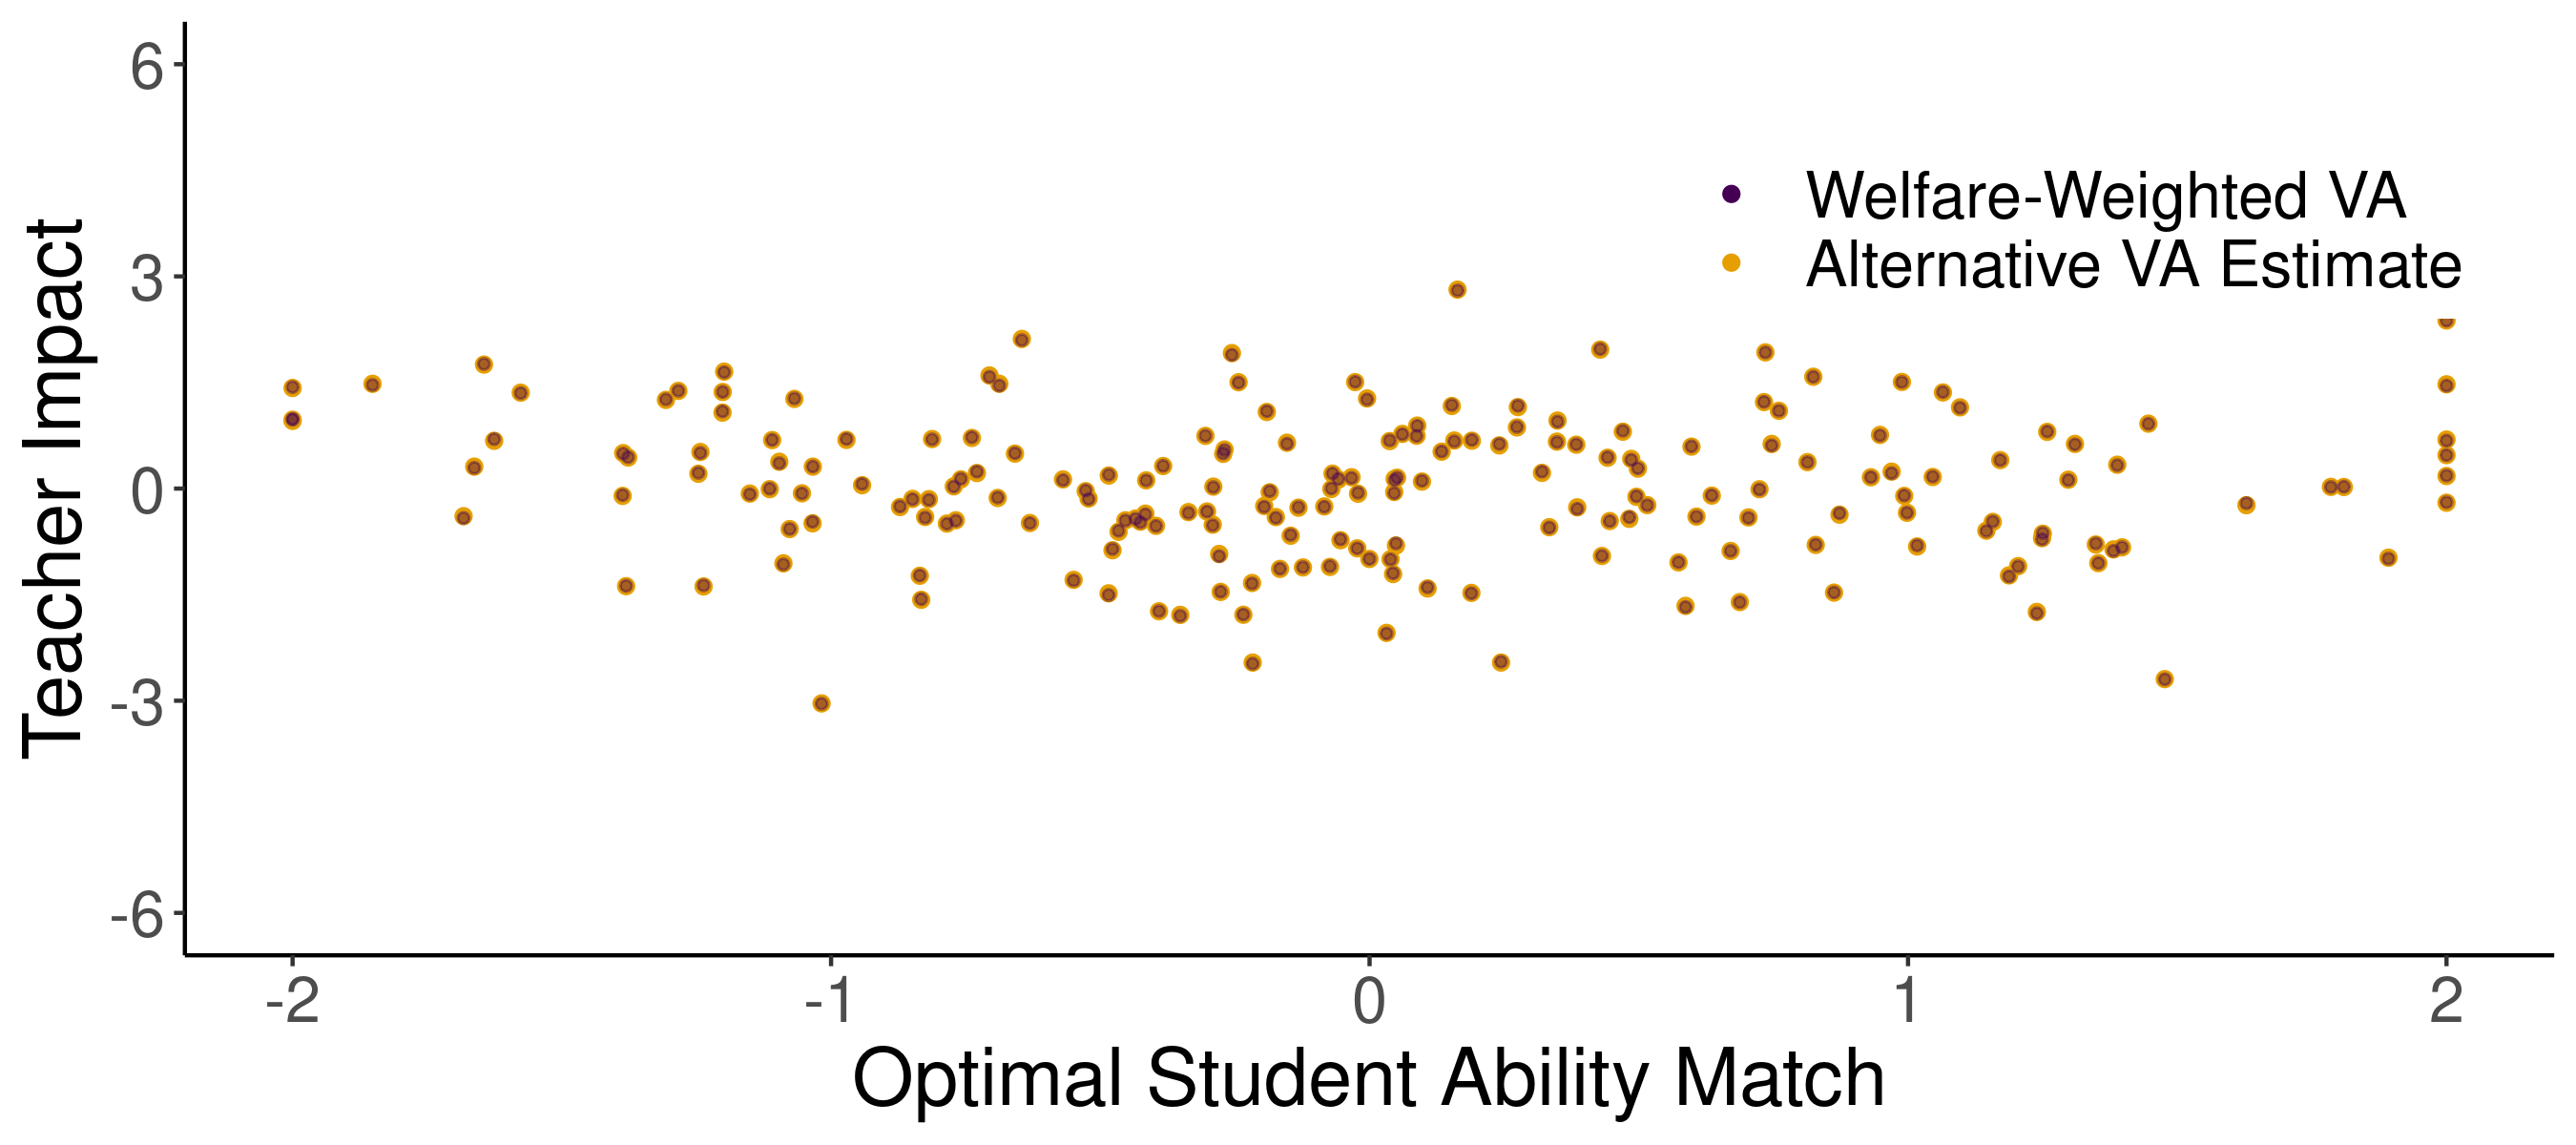
\includegraphics[width=.75\textwidth]{slides/Figures/np_welfare_cent_run_1.png}
\end{figure}

\hyperlink{teacher_ability2}{\beamerbutton{Back}}

\end{frame}


%%%%%%%%%%%%%%%%%%%%%%%%%%%%%%%%%%%%%%%%%%%%%%%%%%%%%%%%
%%%%%%%%%%%%%%%%%%%%%%%%%%%%%%%%%%%%%%%%%%%%%%%%%%%%%%%%

\section*{}
\begin{frame}[noframenumbering]{Only Variation in Match Quality with Average Students}

\hypertarget{st_cent2}{}
\vfill

\begin{figure}
    \centering
 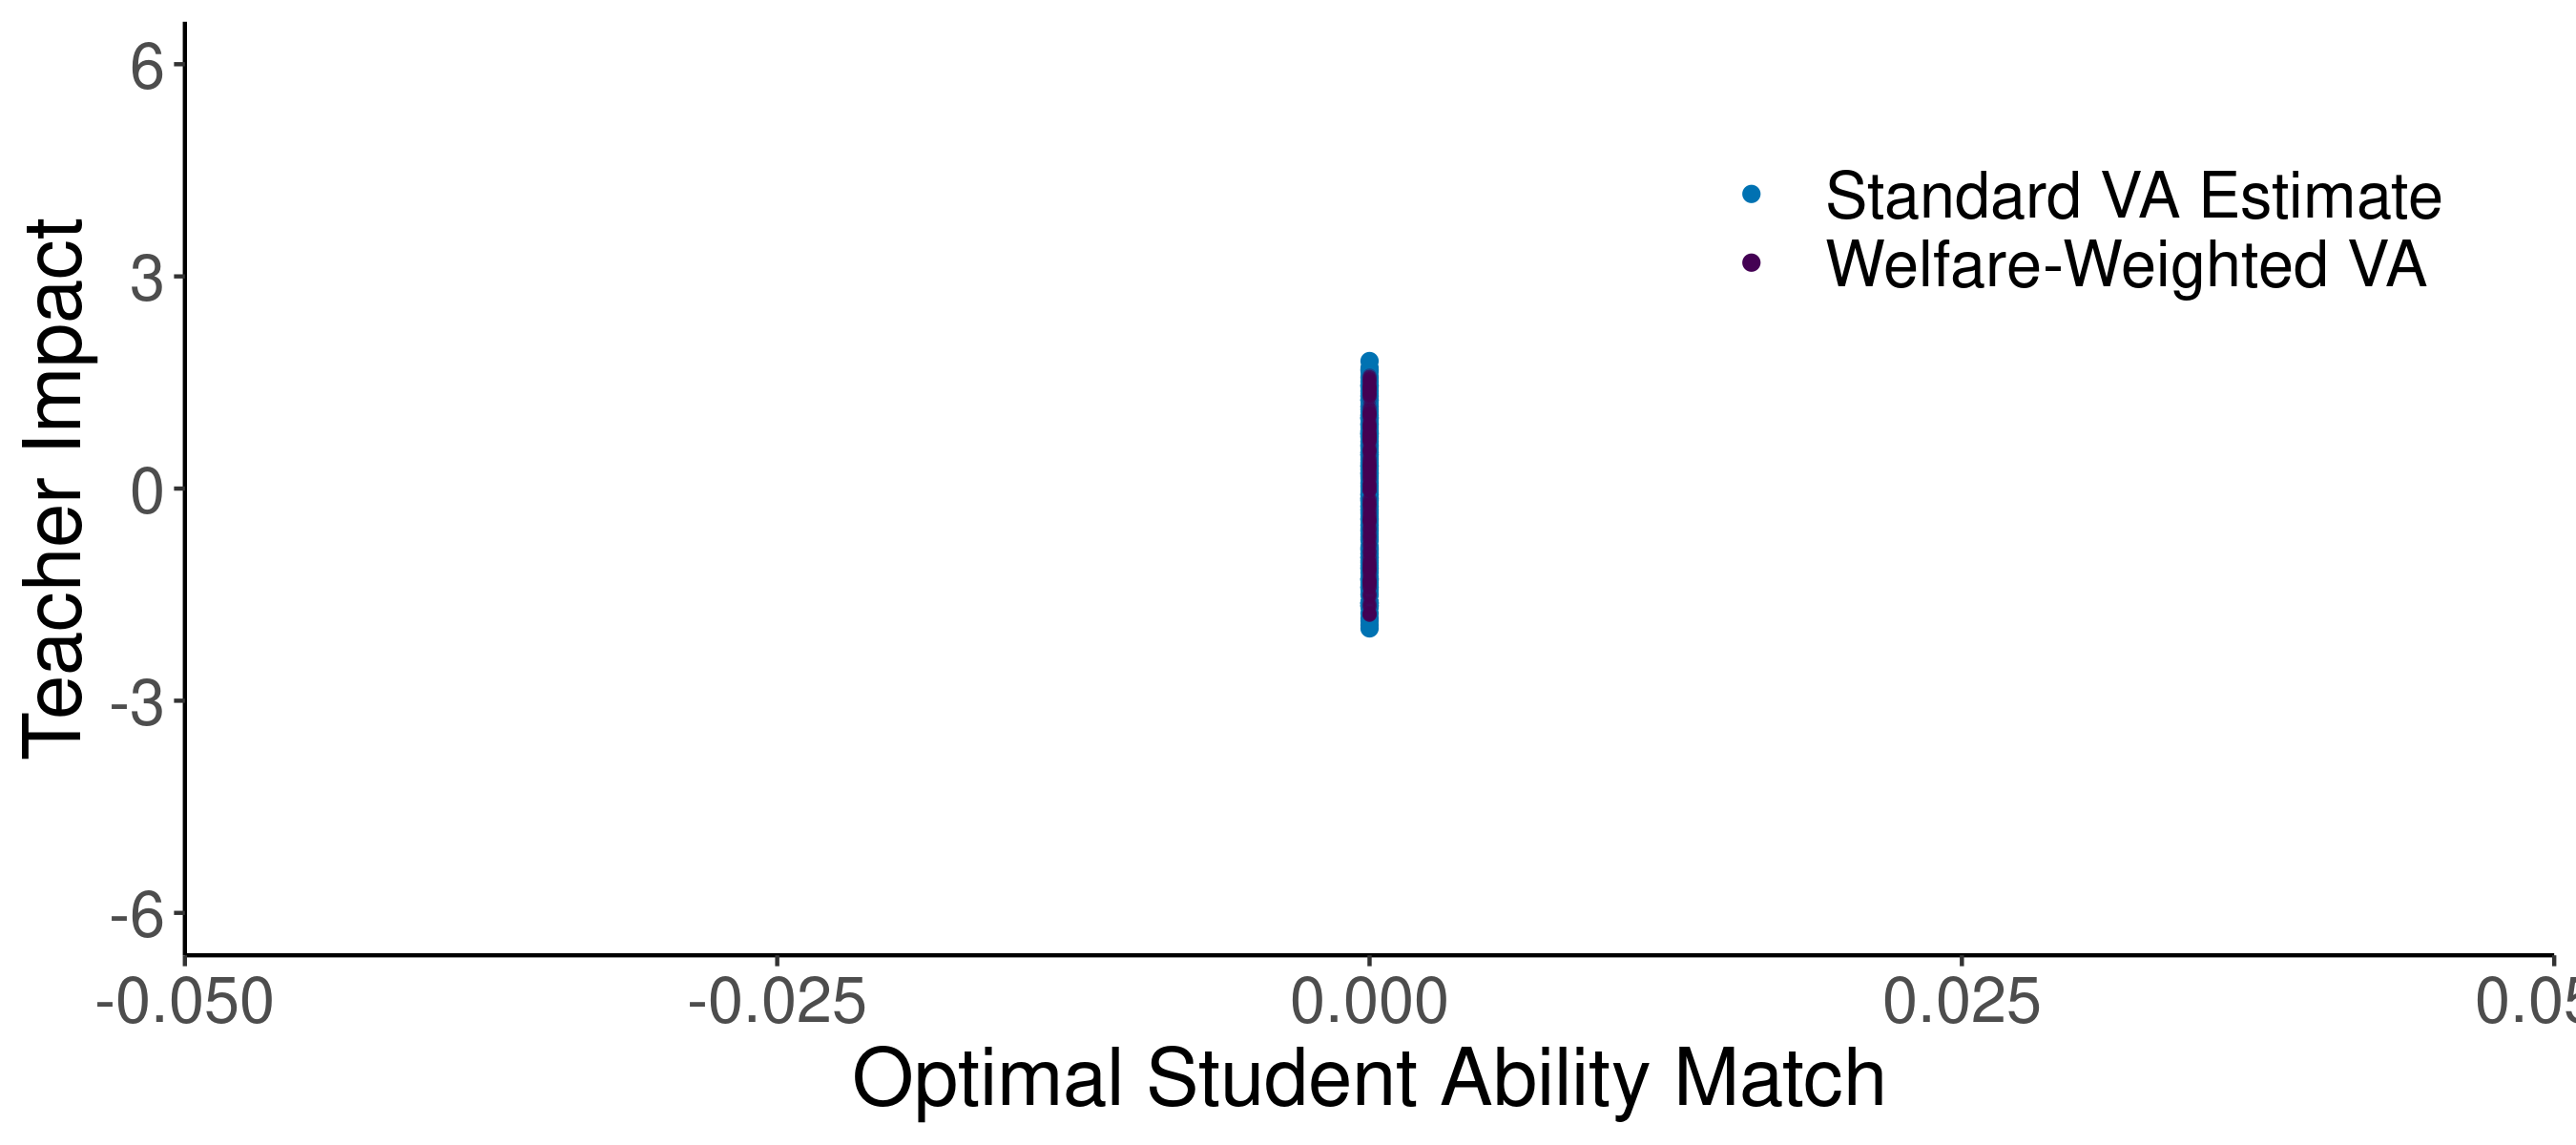
\includegraphics[width=.75\textwidth]{slides/Figures/standard_est_cent_run_2.png}
\end{figure}

\hyperlink{match_average1}{\beamerbutton{Back}}

\end{frame}


%%%%%%%%%%%%%%%%%%%%%%%%%%%%%%%%%%%%%%%%%%%%%%%%%%%%%%%%
%%%%%%%%%%%%%%%%%%%%%%%%%%%%%%%%%%%%%%%%%%%%%%%%%%%%%%%%

\section*{}
\begin{frame}[noframenumbering]{Only Variation in Match Quality with Average Students}

\hypertarget{np_cent2}{}
\vfill

\begin{figure}
    \centering
 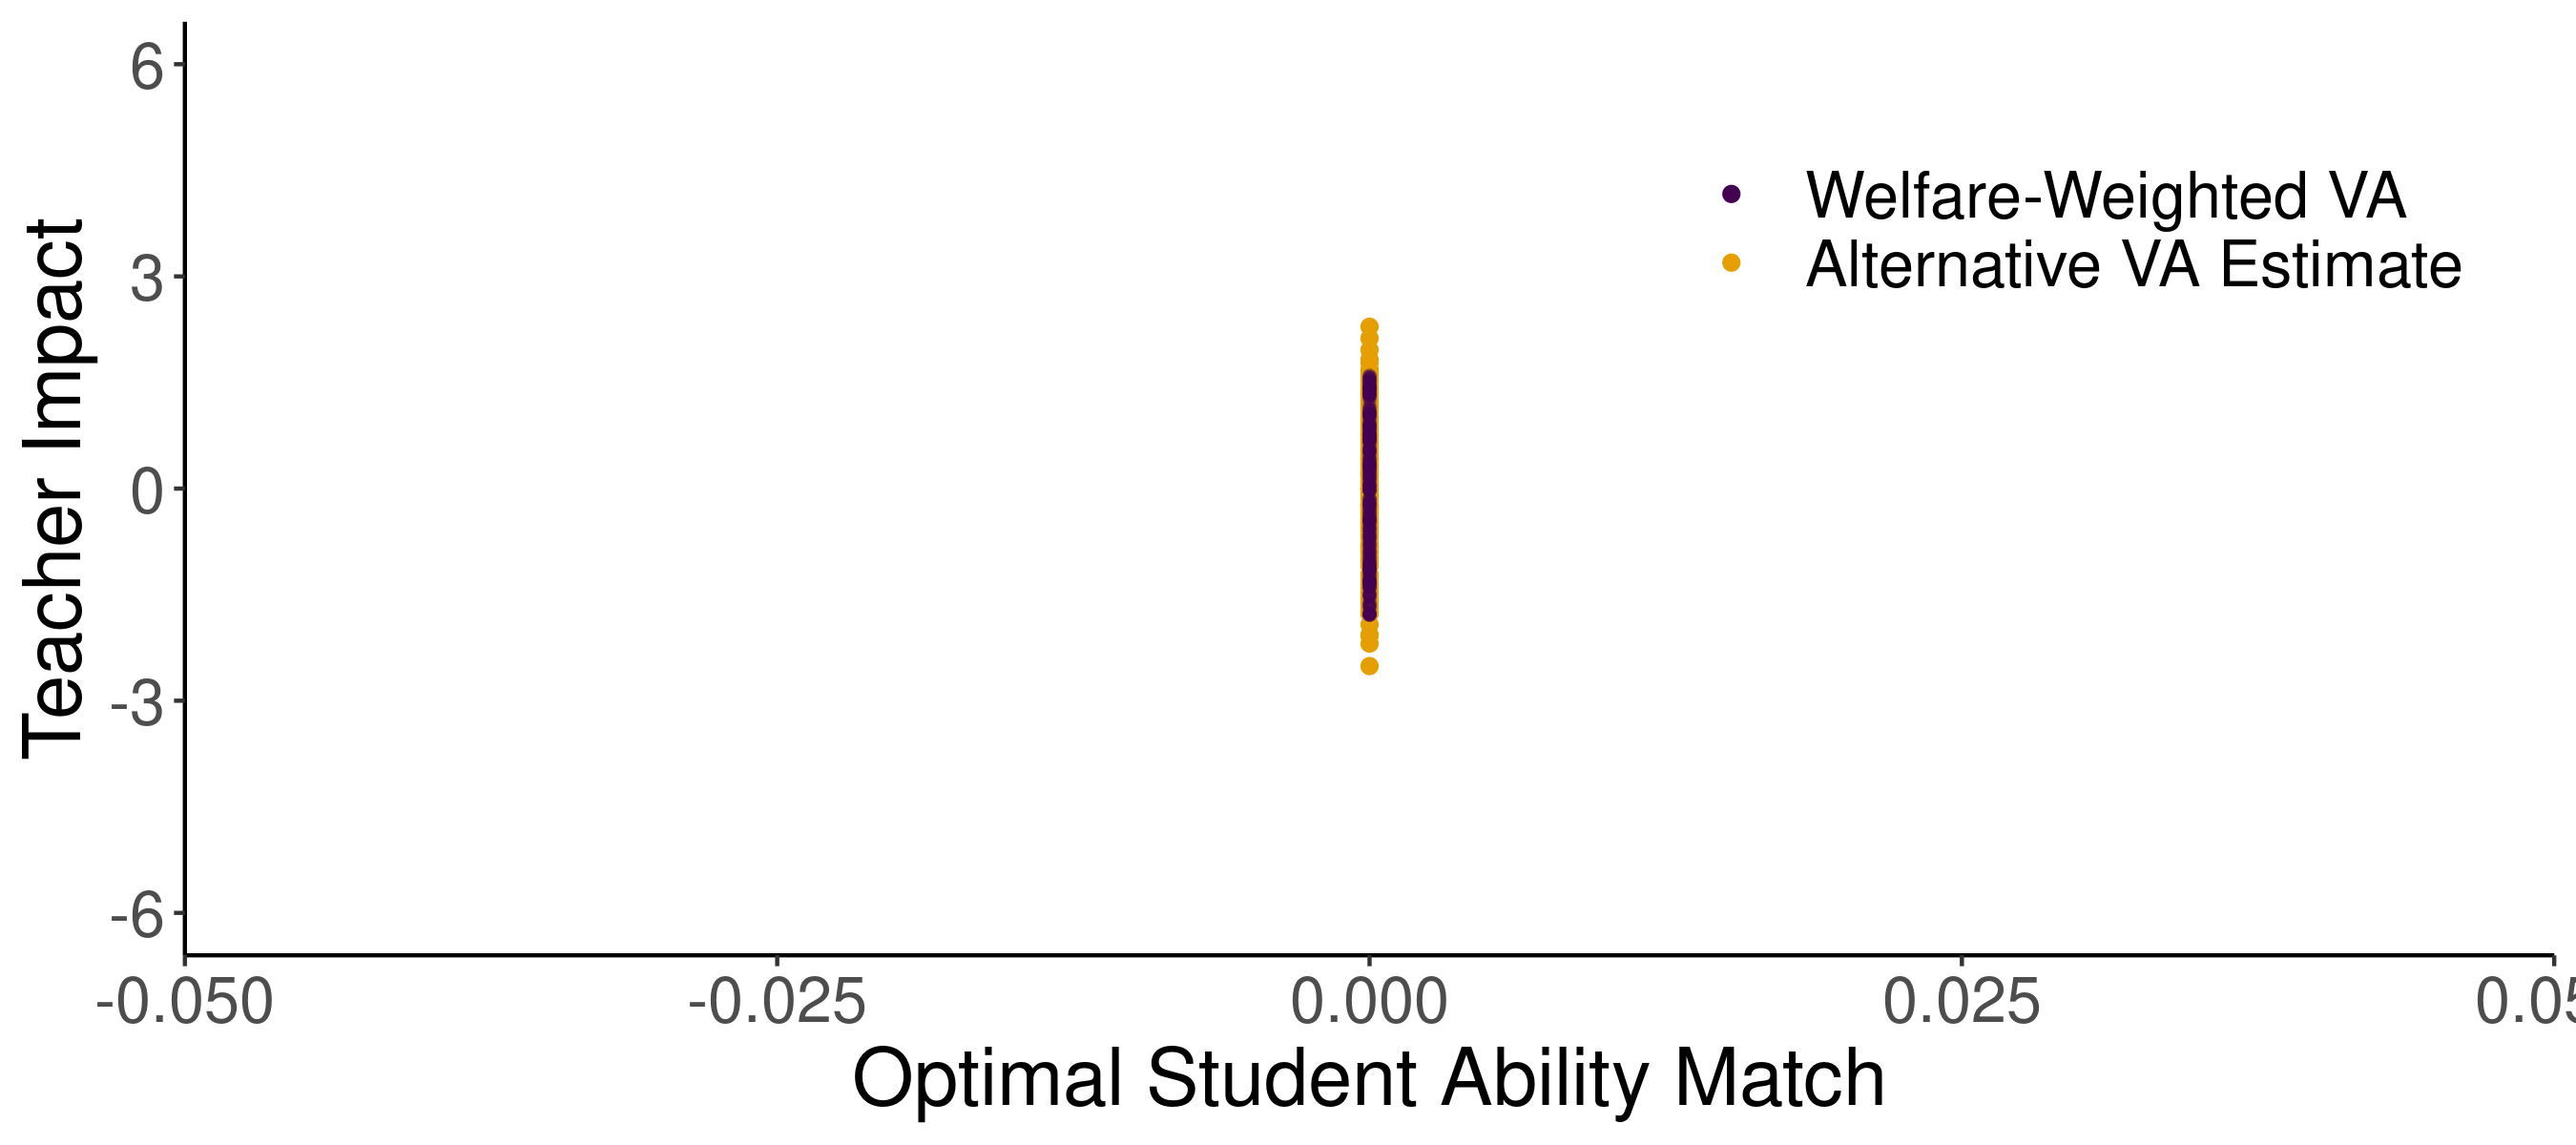
\includegraphics[width=.75\textwidth]{slides/Figures/np_welfare_cent_run_2.png}
\end{figure}

\hyperlink{match_average2}{\beamerbutton{Back}}

\end{frame}


%%%%%%%%%%%%%%%%%%%%%%%%%%%%%%%%%%%%%%%%%%%%%%%%%%%%%%%%
%%%%%%%%%%%%%%%%%%%%%%%%%%%%%%%%%%%%%%%%%%%%%%%%%%%%%%%%

\section*{}
\begin{frame}[noframenumbering]{Only Variation in Match Quality}

\hypertarget{st_cent3}{}
\vfill

\begin{figure}
    \centering
 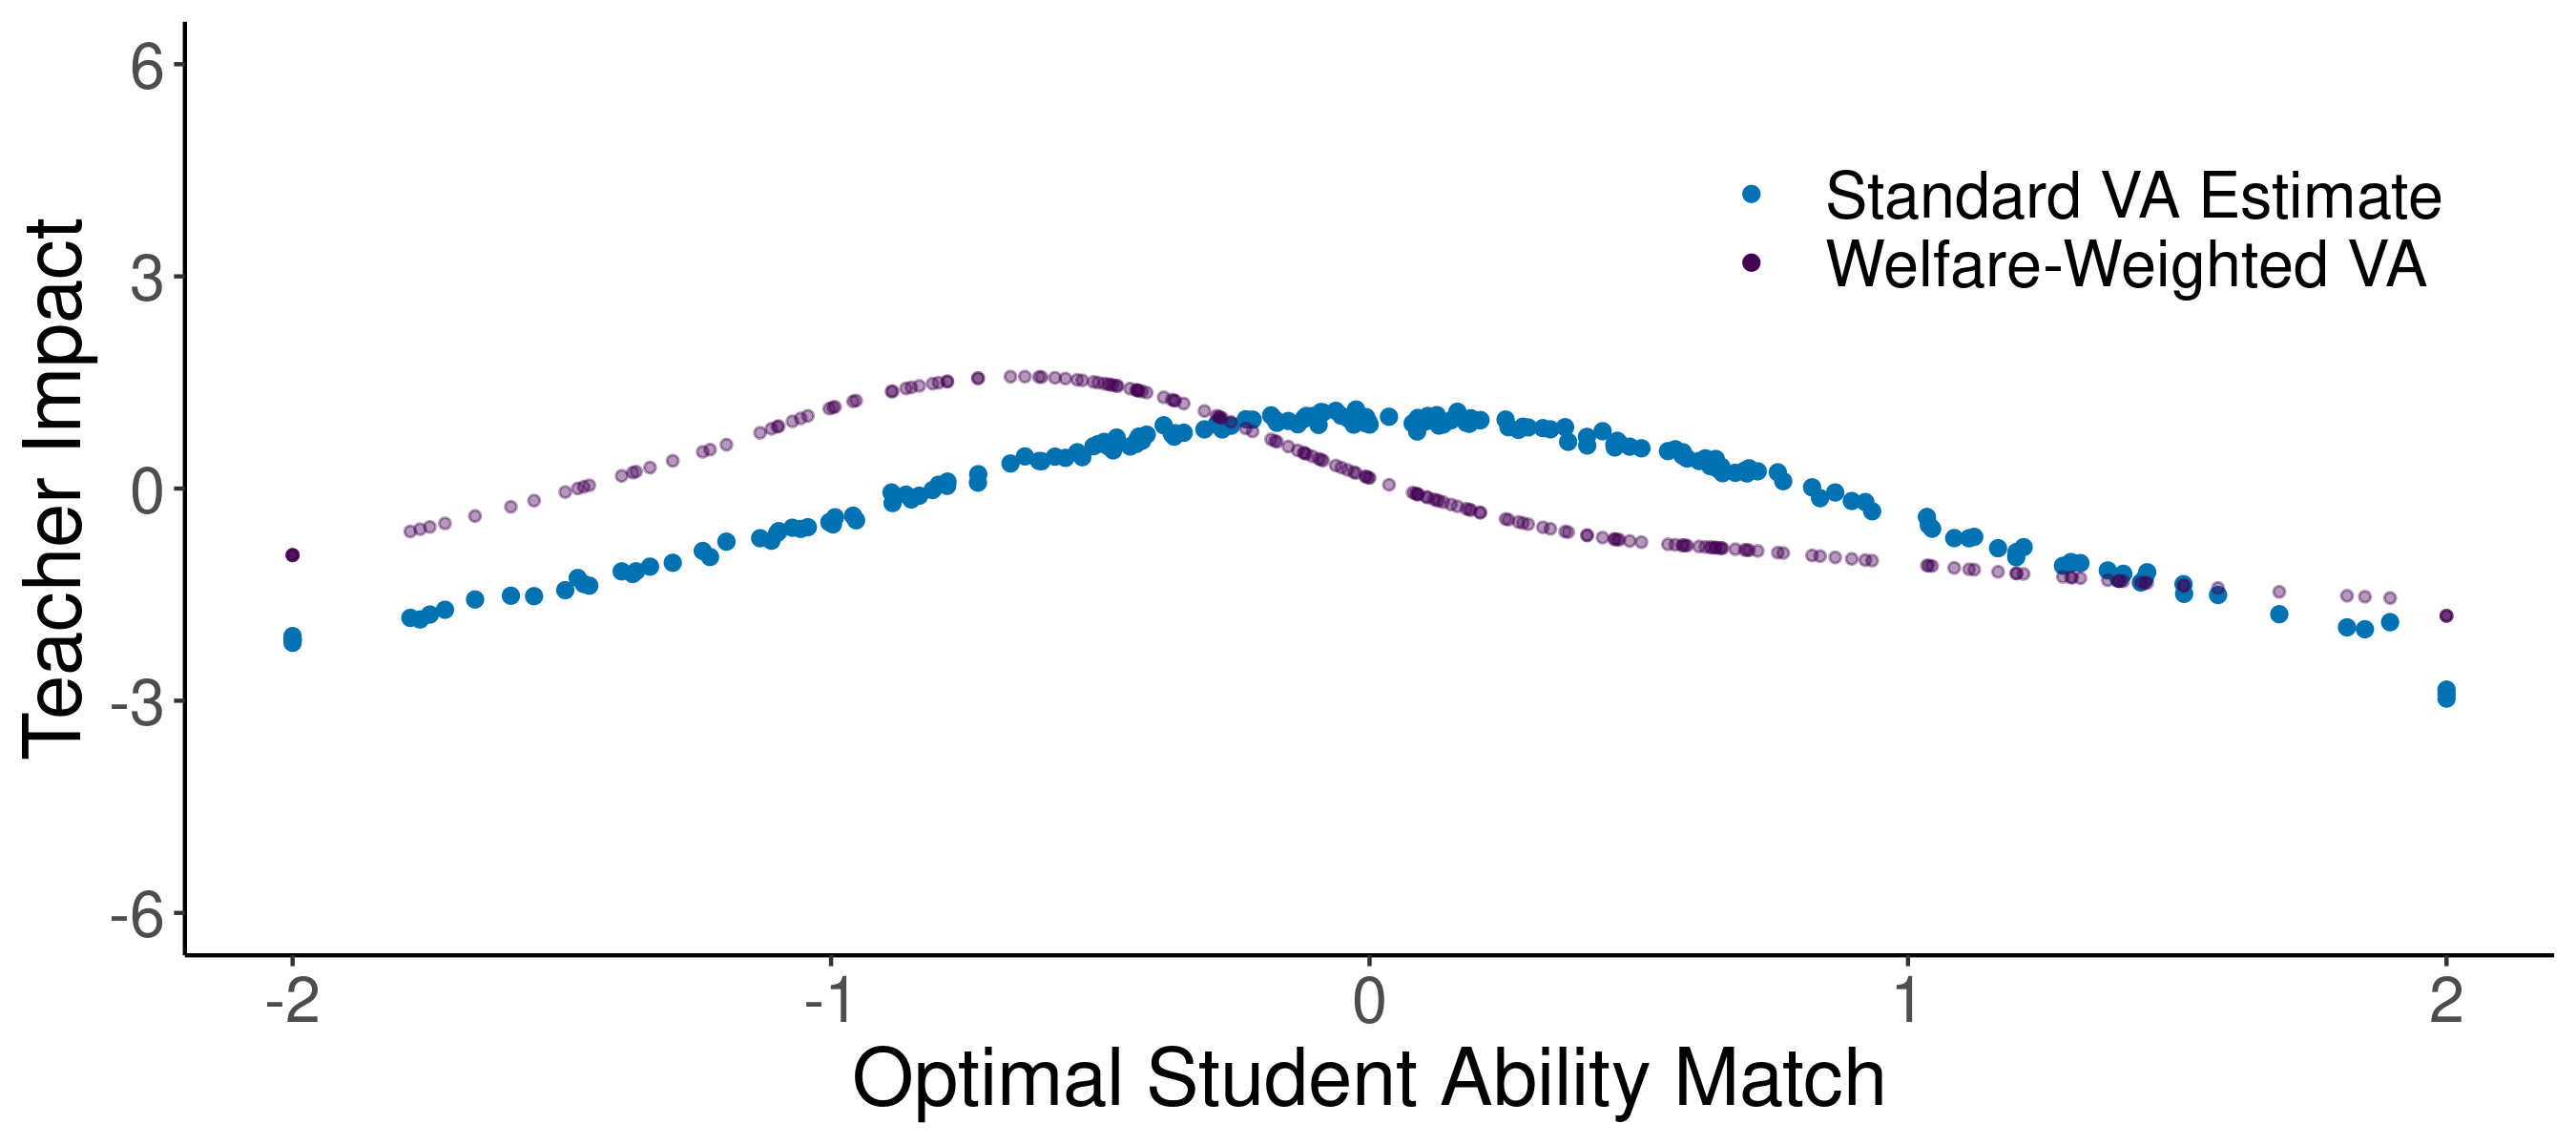
\includegraphics[width=.75\textwidth]{slides/Figures/standard_est_cent_run_3.png}
\end{figure}

\hyperlink{match_quality1}{\beamerbutton{Back}}

\end{frame}


%%%%%%%%%%%%%%%%%%%%%%%%%%%%%%%%%%%%%%%%%%%%%%%%%%%%%%%%
%%%%%%%%%%%%%%%%%%%%%%%%%%%%%%%%%%%%%%%%%%%%%%%%%%%%%%%%

\section*{}
\begin{frame}[noframenumbering]{Only Variation in Match Quality}

\hypertarget{np_cent3}{}
\vfill

\begin{figure}
    \centering
 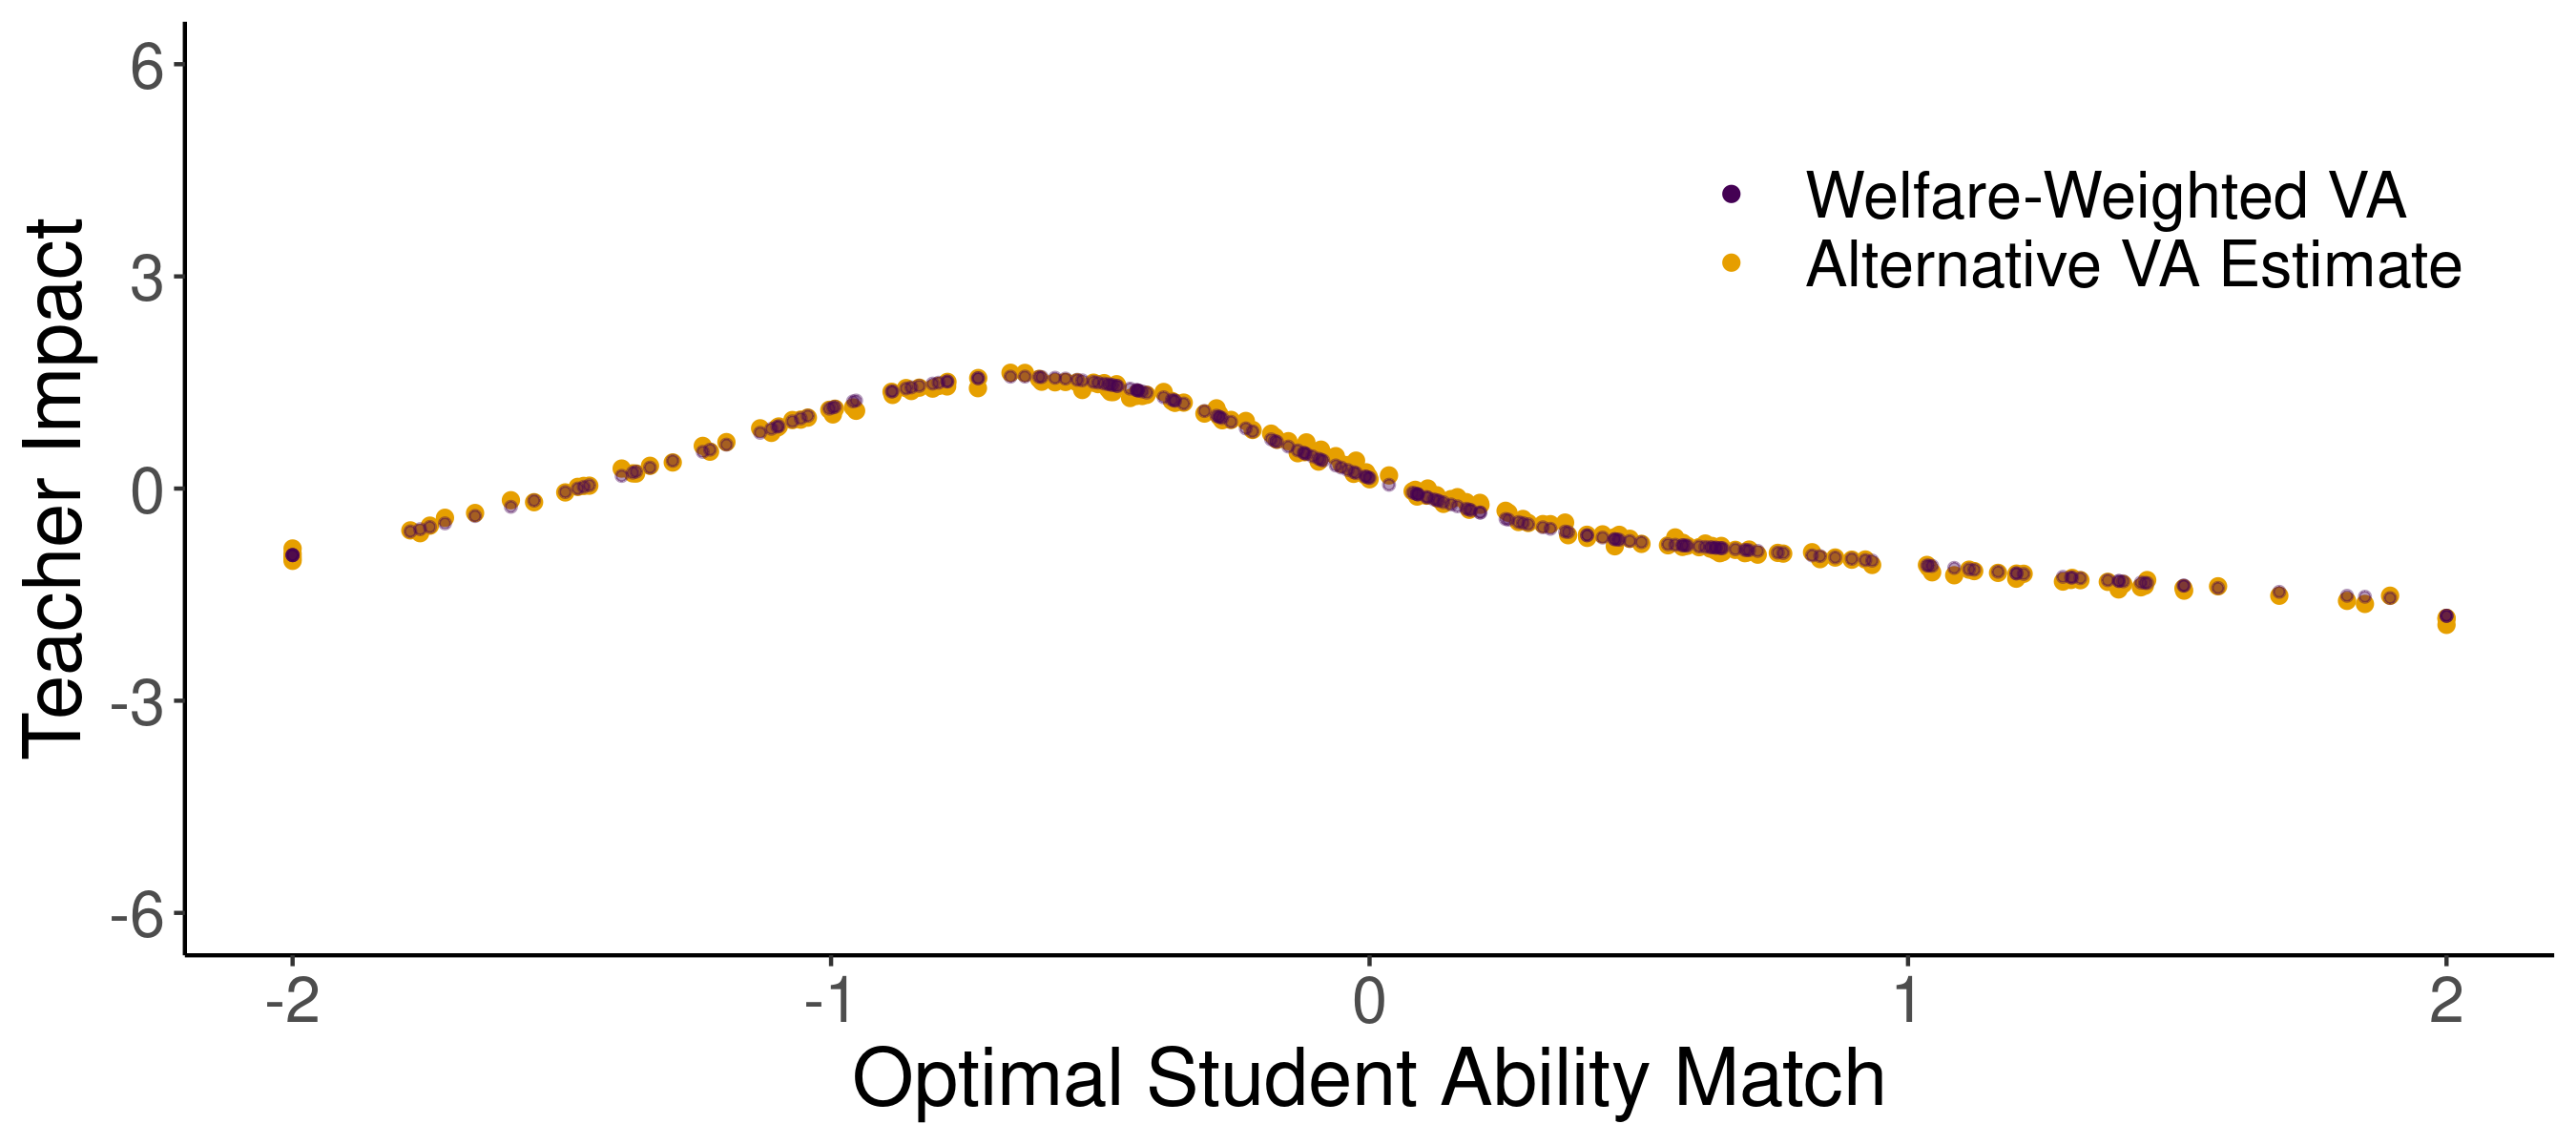
\includegraphics[width=.75\textwidth]{slides/Figures/np_welfare_cent_run_3.png}
\end{figure}

\hyperlink{match_quality2}{\beamerbutton{Back}}

\end{frame}


%%%%%%%%%%%%%%%%%%%%%%%%%%%%%%%%%%%%%%%%%%%%%%%%%%%%%%%%
%%%%%%%%%%%%%%%%%%%%%%%%%%%%%%%%%%%%%%%%%%%%%%%%%%%%%%%%

\section*{}
\begin{frame}[noframenumbering]{Variation in All}

\hypertarget{st_cent4}{}
\vfill

\begin{figure}
    \centering
 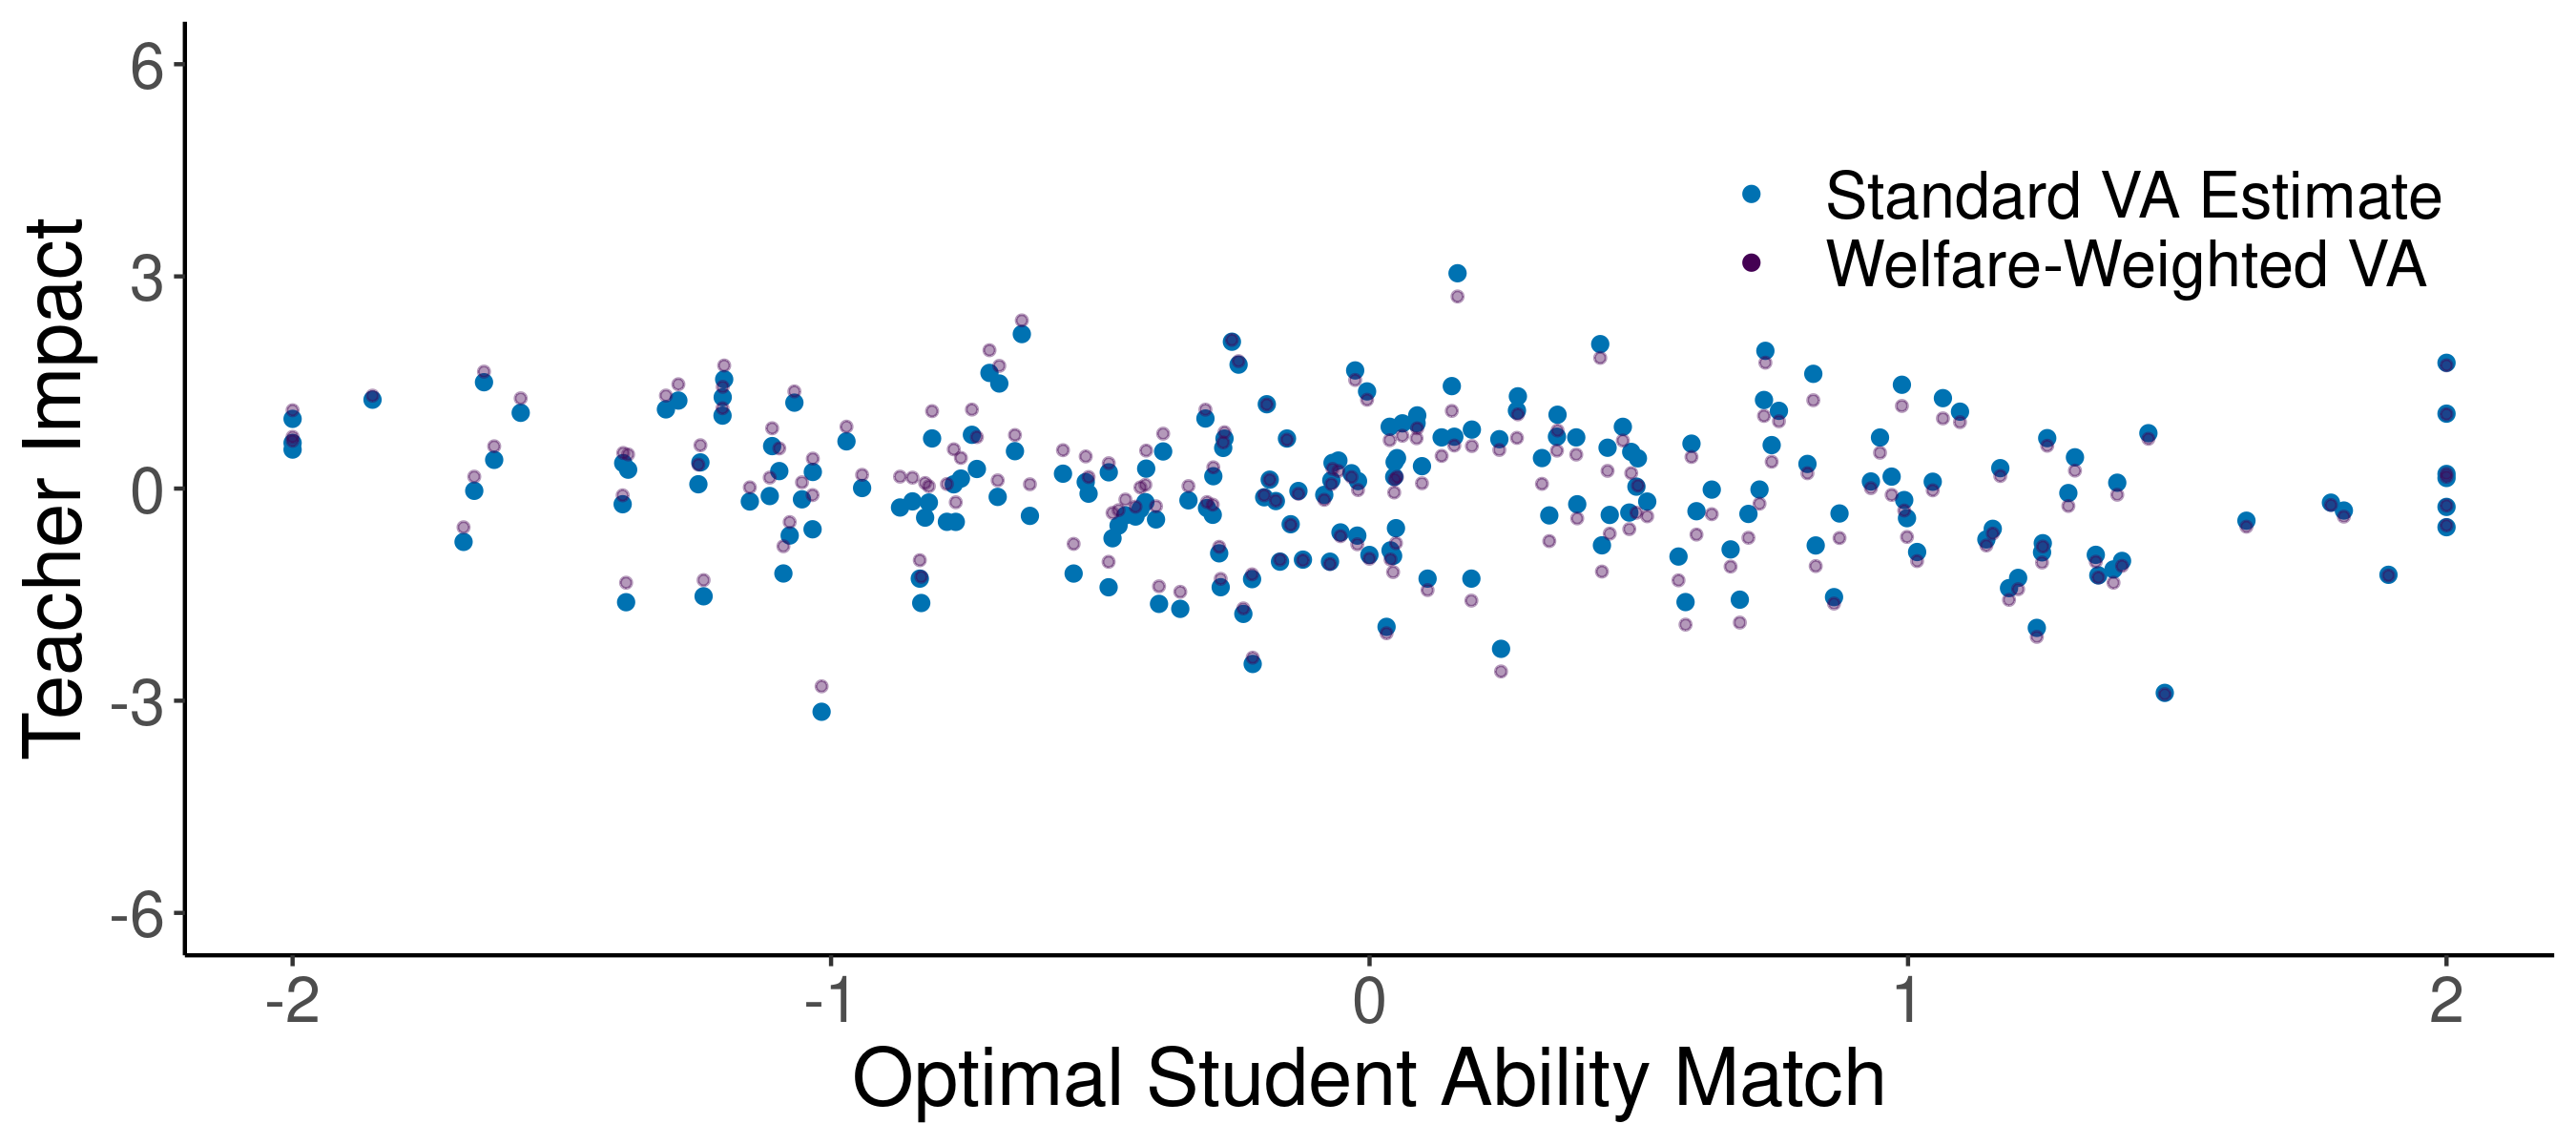
\includegraphics[width=.75\textwidth]{slides/Figures/standard_est_cent_run_4.png}
\end{figure}

\hyperlink{all1}{\beamerbutton{Back}}

\end{frame}


%%%%%%%%%%%%%%%%%%%%%%%%%%%%%%%%%%%%%%%%%%%%%%%%%%%%%%%%
%%%%%%%%%%%%%%%%%%%%%%%%%%%%%%%%%%%%%%%%%%%%%%%%%%%%%%%%

\section*{}
\begin{frame}[noframenumbering]{Variation in All}

\hypertarget{np_cent4}{}
\vfill

\begin{figure}
    \centering
 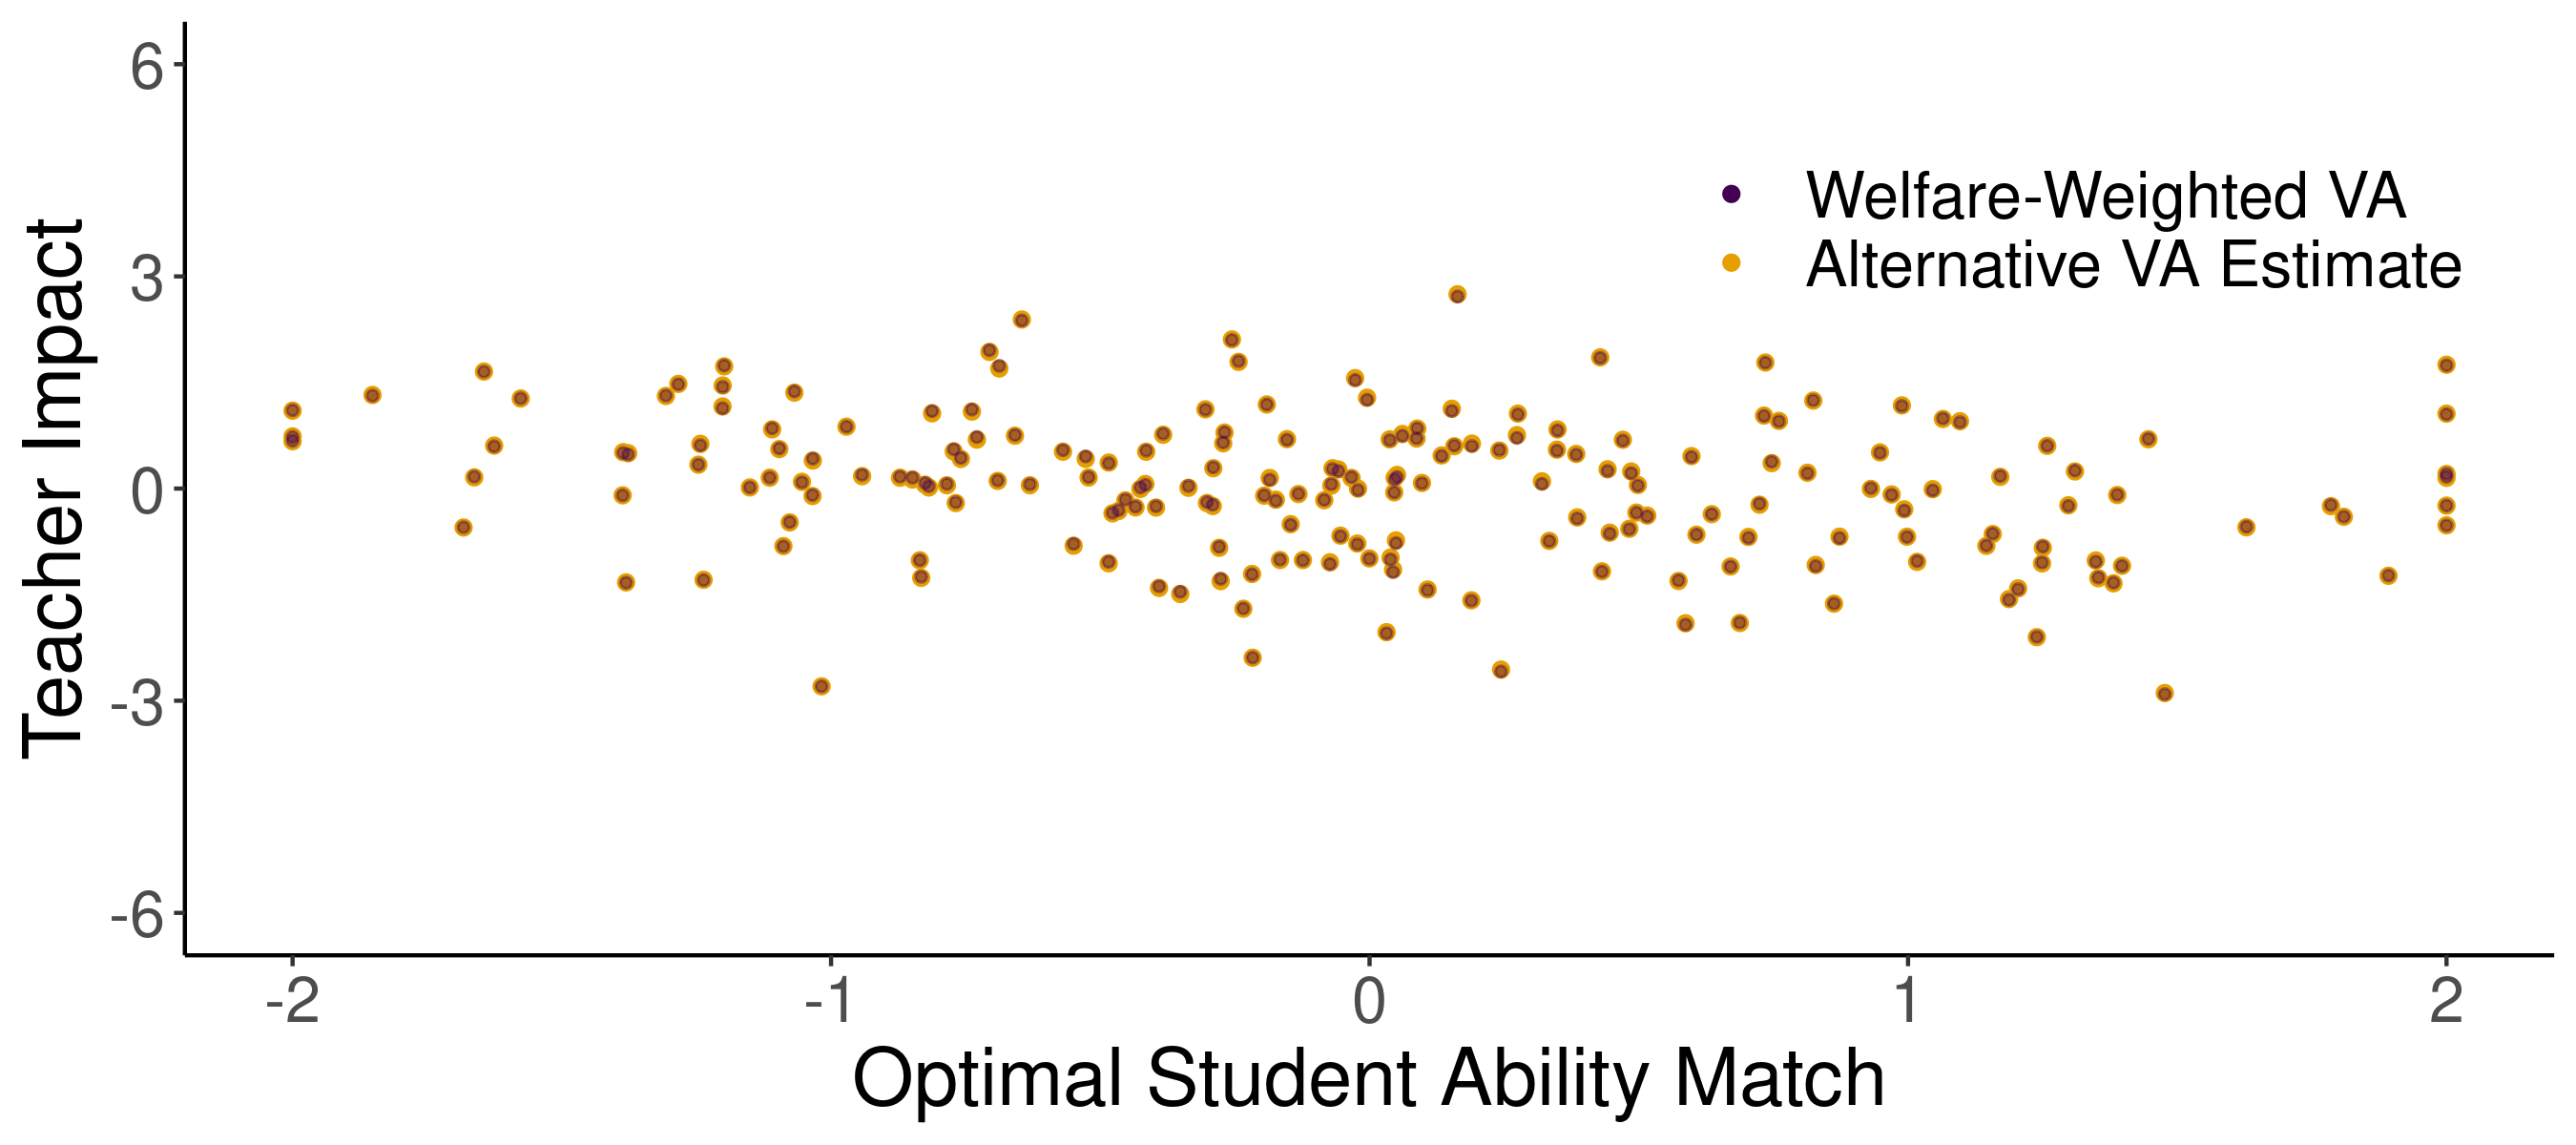
\includegraphics[width=.75\textwidth]{slides/Figures/np_welfare_cent_run_4.png}
\end{figure}

\hyperlink{all2}{\beamerbutton{Back}}

\end{frame}




\end{document}
